\documentclass[a4paper, oneside, onecolumn, 11pt]{article}

\pagestyle{empty}

\usepackage[english]{babel}
\usepackage{graphicx}
\usepackage[space]{grffile}
\usepackage[hyphens]{url}
\usepackage{ltxtable, tabularx, longtable}
\usepackage{listings}
\usepackage{amsmath}
\usepackage{subfig}
\usepackage{cite}

\usepackage{listings}
\usepackage[usenames,dvipsnames]{color}
% This is the color used for MATLAB comments below
\definecolor{MyDarkGreen}{rgb}{0.0,0.4,0.0}

% For faster processing, load Matlab syntax for listings
%\lstloadlanguages{Matlab}%
\lstset{language=Matlab,                        % Use MATLAB
        basicstyle=\small\ttfamily,             % Use small true type font
        identifierstyle=,                       % Nothing special about identifiers
                                                % Comments small dark green courier
        captionpos=b,                           % sets the caption-position to bottom
        commentstyle=\usefont{T1}{pcr}{m}{sl}\color{MyDarkGreen}\small,
        stringstyle=\color{Purple},             % Strings are purple
        showstringspaces=false,                 % Don't put marks in string spaces
        tabsize=5,                              % 5 spaces per tab
        }

\newcommand{\menu}[1]{\textbf{#1}}
\newcommand{\file}[1]{\emph{#1}}
\newcommand{\setting}[1]{''#1''}
\newcommand{\command}[1]{\textbf{#1}}
\newcommand{\control}[1]{\textbf{#1}}

\newcommand{\credit}[1]{\raggedleft \scriptsize Credit:\emph{ #1}}

% Words that should not be hyphenated.
\hyphenation{MATLAB}
\hyphenation{countClassifier}
\hyphenation{splitClassifier}
\hyphenation{deathClassifier}
\hyphenation{SegWSmooth}

\bibliographystyle{IEEEbib}

\title{User guide for Baxter Algorithms 1.6}

\author{Klas Magnusson \\ klasmagnus@gmail.com}

\date{Created: \today}


\begin{document}

\setlength{\extrarowheight}{5pt}

\maketitle

\tableofcontents

\section{Introduction}
The Baxter Algorithms (BA) is a software package for tracking and analysis of cells in microscope images. The software can handle images produced using either transmission microscopy (e.g. bright field, phase contrast, and differential interference contrast (DIC)) or fluorescence microscopy (e.g. wide field, confocal, and light sheet). The analysis of transmission microscopy images is limited to 2D, but 3D stacks of fluorescent images can be processed. In addition to cell tracking, the BA can perform automated analysis of fluorescent histological sections of muscle tissue, and automated analysis of myoblast fusion. The software is written in MATLAB, but it also contains some algorithms written in C++, which are compiled into mex-files.

The software as a whole is presented in \cite{Magnusson16Thesis} and an example of how the software can be used to analyze muscle stem cell (MuSC) behavior is found in \cite{Gilbert10Elasticity}. The data association algorithm used to generate cell tracks is described in \cite{Magnusson12Viterbi, Magnusson15Viterbi}. The software has shown outstanding performance compared to other software in the ISBI Cell Tracking Challenges of 2013, 2014, and 2015 \cite{Maska14Benchmark, Ortiz15Challenge, Ulman17Objective}.

\section{Quick guide}
I am aware that many users will not take the time to read this manual when they start using the software, and therefore I have put together a quick guide. It will be helpful when you start using the program and when you try to remember how to do things, but please try to read the entire manual at some point. It will save you time in the long run.

\begin{enumerate}
\item Download the software from\\ \url{https://github.com/klasma/BaxterAlgorithms}.
\item Install the software, or run the source code in MATLAB.
\item Put your image sequences (or individual images) in separate folders and put these folders in an experiment folder.
\item Open the experiment folder in BA.
\item Load appropriate settings or enter them manually.
\item If you have acquired multiple channels, you need to specify the settings \setting{channelNames} and \setting{channelTags} to tell the program how to identify the different channels.
\item If you have multiple channels, you need to set the colors of the different fluorescent channels using the menu option \menu{Settings/\allowbreak Set fluorescence display}. You need to select the advanced option in the level menu for this menu option to show up.
\item Edit the segmentation settings if necessary, using the menu option \menu{Settings/\allowbreak Set segmentation parameters}.
\item Start the processing using the menu option \menu{Automated/\allowbreak Track}. For transmission microscopy of cells in microwells, you first need to run \menu{Automated/\allowbreak Stabilize}, and possibly also \menu{Automated/\allowbreak Cut microwells}.
\item Review the tracking results using the menu option \menu{Manual/\allowbreak Track Correction} and edit the tracks and/or the outlines if you think that it is necessary for the analysis that you want to do.
\item Analyze the tracking results. The graphical user interface (GUI) under \menu{Analysis/\allowbreak Cell Analysis GUI} shows how properties of individual cells evolve over time, and the GUI under \menu{Analysis/\allowbreak Population Analysis GUI} shows cell properties averaged over time.
\item Develop your own analysis scripts using MATLAB. The most important classes to know about are:
\begin{itemize}
\item Cell
\item Blob
\item ImageData
\end{itemize}
The most important functions to know about are:
\begin{itemize}
\item LoadCells
\item SaveCells
\end{itemize}
The functions are documented with comments in the files, and the documentation can be displayed by typing \command{doc} or \command{help} followed by the function name in the MATLAB command window.
\end{enumerate}

\section{Video tutorials}
In the YouTube playlist \url{https://tinyurl.com/ba-tutorials} there are 16 video tutorials which give you step by step instructions on how to perform different tasks in the program. The topics of the tutorials are listed below.

\begin{enumerate}
\item Introduction
\item Installing and running the program
\item Image stabilization
\item Cutting of microwells
\item Opening multichannel data
\item Opening 3D data
\item Tracking in bright field microscopy
\item Tracking in fluorescence microscopy
\item Tracking in 3D fluorescence microscopy
\item Track correction
\item Segmentation correction
\item Data analysis
\item Writing analysis scripts
\item Fiber analysis
\item Myotube fusion analysis
\item Loading segmentations
\end{enumerate}

\section{Installation}
\label{sec:installation}
The program is publicly available as a git repository on \url{https://github.com/klasma/BaxterAlgorithms}. The software is available in the form of source code and deployed applications for Windows and Mac. All forms can be downloaded by clicking on the \control{releases} tab and expanding the \control{Assets} dropdown under the latest release. If you have git installed, you can also clone the git repository to get access to the version controlled source code. The deployed software only runs on 64-bit Windows and Mac systems, but the source code be executed in MATLAB on other systems after compiling C++ components as described in Section \ref{sec:compile}.

\subsection{Running the deployed application}
\label{sec:run-deployed}
If you do not have a MATLAB licence, you can run a deployed version of the program. The deployed versions can be found on the \control{releases} tab on https://github.com/klasma/BaxterAlgorithms. There, you expand the \control{Assets} dropdown under the latest release, and download the installer for your operating system. The installers for Windows and Mac are called \file{BaxterAlgorithmsInstaller\_win64.exe} and \file{BaxterAlgorithmsInstaller\_maci64.app} respectively. To run the deployed program, you need the MATLAB Compiler Runtime (MCR). The correct version of the MCR will be downloaded and installed during the BA installation, if it is not already installed. On Windows, text output will be written to a dedicated MS-DOS Command Window which is opened when you start the program by clicking on the icon on the desktop or in the start menu. On Mac, you can open the application by clicking on the icon, but to get text output, you need to start the program from the terminal as described in Section \ref{sec:mac-terminal}.

\subsection{Running the source code}
\label{sec:source}
If you have MATLAB installed, you can execute the source code directly in MATLAB. The BA has been tested in MATLAB 2015b and 2018b. The software should work for those versions and all versions in between. Later versions are likely to work as well, but minor changes to the code may be necessary as MATLAB syntax is not always backward compatible. In addition to MATLAB, you also need the tool boxes for Image Processing, Optimization, Parallel Computing, and Statistics. All the necessary toolboxes are usually included in academic licences. If you have git, the easiest way to get the source code is to clone the git repository https://github.com/klasma/BaxterAlgorithms. Otherwise, you can download the source code from the repository website by clicking on the \control{releases} tab and expanding the \control{Assets} dropdown under the latest release. In MATLAB, you need to open the file \file{BaxterAlgorithms.m} and run it by pressing the run button in the MATLAB editor. When you press \command{run}, MATLAB might say that the file is not found in the current folder, and in that case you press the button to change folder. The first time you run the program, there will be a dialog saying that the program needs to modify a file called \file{javaclasspath.txt}.

\section{Image data format}
\label{sec:image-data-format}
The program is designed to process 8 bit or 16 bit gray scale images. The program can also process color images with 3 RGB channels, but that is done by internally converting the color image to gray scale. The program recognizes the file extensions tif, tiff, png, jpg, and jpeg. I recommend that you use tif-files, because most of the testing has been done with tif-files, and some read operations are faster when that file format is used. The images need to be organized into individual folders for the different image sequences (even if an image sequence only has a single image). These folders are then put into an experiment folder. The filenames in an image sequence folder do not have to follow any particular convention as long as the files are in the correct order when alphabetized. To ensure this, you need to pad numbers with zeros as in \file{image\_02.tif}, so that \file{image\_10.tif} is not put before \file{image\_2.tif}. The program will save meta data and algorithm parameters associated with the image sequences in a file named \file{Settings.csv} in the experiment folder. Tracking results and other data created by the program will be stored in a folder named \file{Analysis} inside the experiment folder.

\subsection{3D volumes}
If you have 3D $z$-stacks, you can either save each $z$-stack as a tif-stack or save the $z$-slices as individual images. If you save individual images, you need to make sure that the alphabetical order of the files is such that the time points are in alphabetical order and such that the $z$-slices in each block of files are ordered from the first slice to the last slice. To make the program load the 3D volumes correctly, you need to specify the settings \setting{numZ} and \setting{zStacked} described in Table \ref{tab:image-settings}.

\subsection{Multiple channels}
If multiple channels have been acquired, for example if there are fluorescent channels in addition to a transmission microscopy image, all channels should be put in the same image sequence folder. This requires that each channel has a part of the file name which is specific to that channel. To make the program identify the channels correctly, you need to set the \setting{channelNames} and \setting{channelTags} settings as described in Section \ref{sec:settings-fluorescence}.

\section{Running the program}
You start the program by either double clicking the icon of the deployed application or by running \file{BaxterAlgorithms.m} in MATLAB as described in Section \ref{sec:source}. Starting the program opens the window shown in Figure \ref{fig:main-GUI}.

\begin{figure}[!ht]
\begin{center}
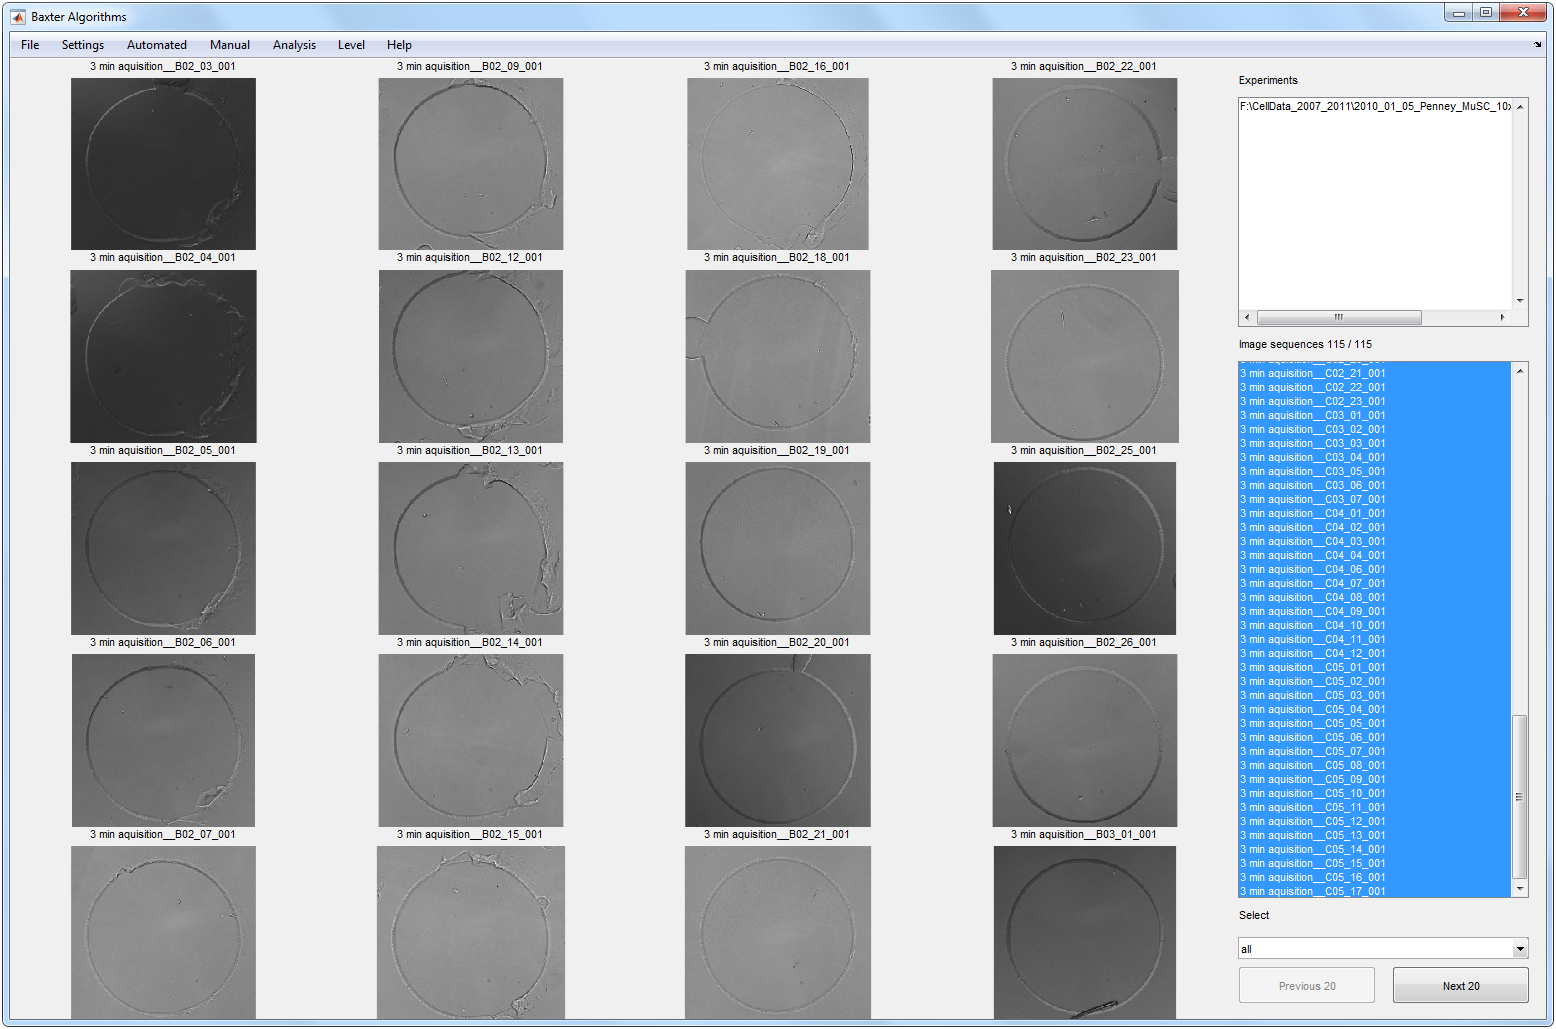
\includegraphics[width = \columnwidth]{figures/mainGUI}
\credit{Penney Gilbert, Stanford University}
\caption{The main GUI window, from which all other GUIs can be opened.}
\label{fig:main-GUI}
\end{center}
\end{figure}

\subsection{Text output in the deployed application for Mac}
\label{sec:mac-terminal}
During execution, the program will produce text output with progress indications, results, and error messages. When the source code is executed in MATLAB, the output is sent to the Command Window. When the deployed application is executed on Windows, the the output is sent to an MS-DOS Command Window which is opened together with the program. When the program is executed on Mac, you will not get any text output if you start the program by clicking on the icon. In order to get text output on Mac, you need to start the program from the terminal, using a shell script which is located inside the .app-folder associated with the program. The shell script takes the path of the installed Matlab Compiler Runtime (MCR) as an input argument. To start the program in this way, you first open a terminal window. One way to do that is to click the magnifying glass in the upper right corner of the screen, and typing \command{Terminal} into the search field. You run the shell script by entering the full path of the shell script followed by the full path of the MCR. If you installed both the BA and the MCR in the default locations, you enter \command{/\mbox{Applications}/\allowbreak BaxterAlgorithms/\allowbreak \mbox{application}/\allowbreak run\_BaxterAlgorithms.sh \allowbreak/\mbox{Applications}/\allowbreak MATLAB/\allowbreak\\ MATLAB\_Compiler\_Runtime/\allowbreak v95/}.

\subsection{Opening experiments}
You open an experiment by clicking on \menu{File/\allowbreak Open experiment} and selecting the desired experiment folder. If you have a single image sequence stored in a folder, you must put this folder into an experiment folder and open that folder in the program. You can open multiple experiment folders by either selecting multiple folders in the experiment opening dialog or by clicking \menu{File/\allowbreak Add experiment}. Opening new experiments using \menu{File/\allowbreak Open experiment} will automatically close all open experiments.

\subsection{Browsing through image sequences}
Once an experiment is open, you can see the first images of the image sequences by selecting their file names in the list box labeled \control{Image sequences}. Different subsets of the image sequences can be selected using the dropdown menu labeled \control{Select}. If more than 20 image sequences are selected, you can browse through them using the buttons \control{Next 20} and \control{Previous 20}.

\subsection{Performing tasks}
All tasks that can be performed on the image sequences can be found in the menus of the main window. Clicking such a menu will in general perform the corresponding task on the image sequences that have been selected.

\subsection{User levels}
The menus and the settings of the program have been classified into the three different levels \setting{basic}, \setting{advanced}, and \setting{development}. This has been done to guide users to the most important functions and settings, and to hide some of the more advanced functionalities from users how are learning the software. You can select a user level in the \menu{Level} menu in the main GUI. The GUIs found under \menu{Settings/Settings} and \menu{Setting/Set segmentation parameters} also have \menu{Level} menus, and they are independent from the one in the main GUI.

The basic level has all the important functions and settings necessary to process image sequences. The advanced level has additional functions and settings which provide higher performance and flexibility. The development level has functions that developers may find interesting. These functions and settings are either experimental or have very limited utility. Functionalities at the development level may also not work properly in the current version of the program, and may be removed in a future version. Avoid using these functionalities if you do not need them.

\subsection{Players}
\label{sec:players}
Many of the functions in the menus will open different players, where the image sequences can be played and processed or analyzed. These players all share the same structure, but they have different buttons and menu options. The simplest player is found under \menu{Manual/\allowbreak Play} and only plays the image sequences. Before any analysis is done, it is good to look at the image sequences in this player to make sure that all the image sequences are saved in the correct format and that all image settings are correct.

\subsubsection{Zooming and panning}
All of the players that show images allow you to zoom and pan. You zoom by holding down the left mouse button somewhere in the image and dragging to create a rectangle around the region that you want to display. You zoom out by right-clicking. When you have zoomed in, you can pan around in the image by holding down the space bar and dragging with the left mouse button down. You can also toggle panning by pressing \command{m}. You press \command{m} once to enable panning and then again to disable it. That can be useful if you are working on a laptop which disables the touchpad when you hold down space. In the players for manual correction, zooming is turned on by selecting the zoom tool, but the panning tool is always turned on so that you can move around in the image quickly. In other players, zooming and panning are always turned on.

\subsection{Visualizing 3D data}
When you view 3D data in a player, as in Figure \ref{fig:3D-players}, an additional control panel will appear to the right of the image. That control panel has controls which determine how the 3D data is displayed. In the \control{display} dropdown menu, you can select what 3D views you want to look at. The default is to show the $xy$-view, but you can also show the $xz$-view or the $yz$-view, or all views at once as in Figure \ref{fig:3D-players}. By default, the players will show maximum intensity projections through the 3D volume, but you can also select to show individual slices by un-checking the checkboxes \control{x proj.}, \control{y proj.}, and \control{z proj.}. Once you are displaying individual slices, you can select which slice to display using the text boxes and sliders labeled \control{x}, \control{y} and \control{z}. You can also select slices in the images by shift-clicking or clicking with the middle mouse button, in one of the other 3D views. Lines in the other 3D views show the locations of the selected slices. Controls which have no effect on the current visualization are disabled. You can zoom and pan in the different 3D views, just as in 2D data. When you have zoomed in, maximum intensity projections will be computed over the zoomed in volume and not over the whole $z$-stack.

\begin{figure}[!ht]
\begin{center}
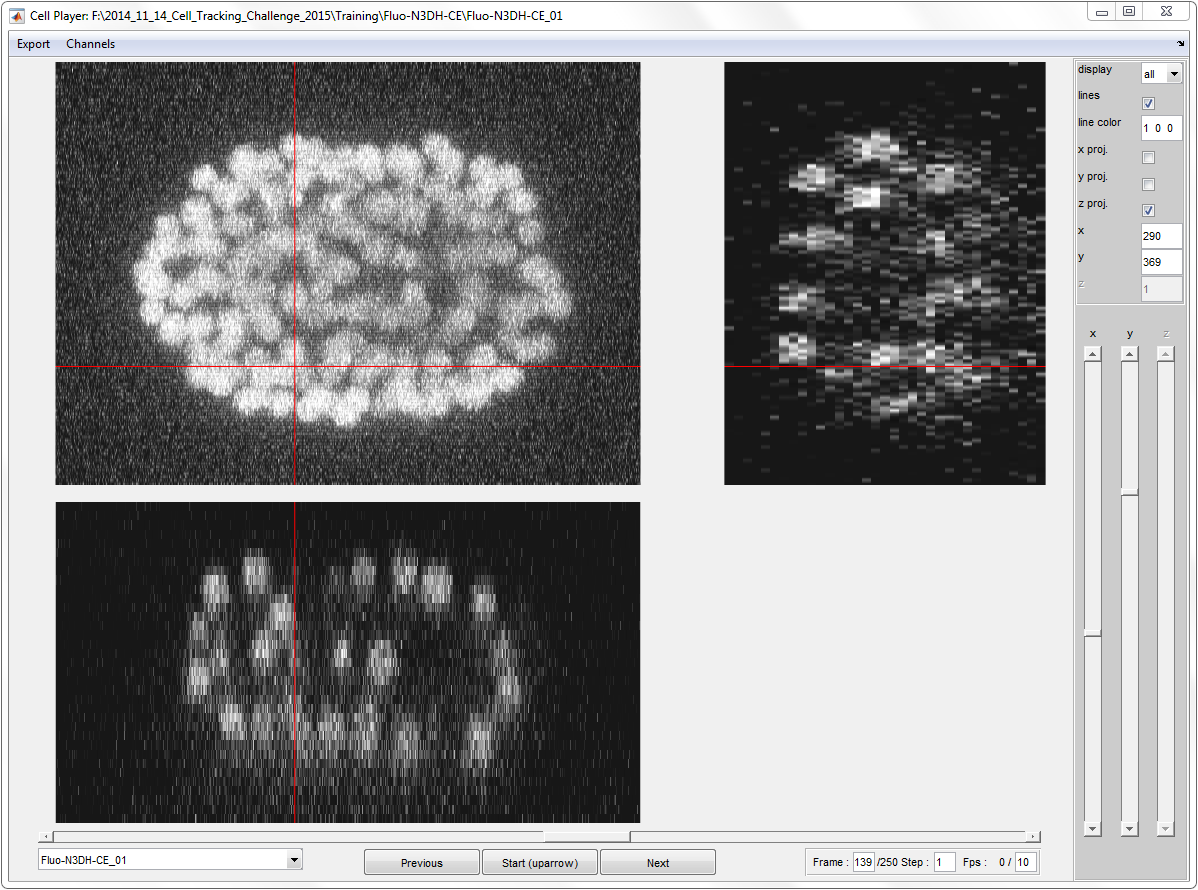
\includegraphics[width = \columnwidth]{figures/3Dplayers.png}
\caption{Controls which are used to change how 3D data is displayed.}
\label{fig:3D-players}
\end{center}
\end{figure}

\subsubsection{Displaying multiple channels}
By default, the players will display all channels as a single merged image, but under the menu option \menu{Channels}, you can select what channels you want to include in the merge. The image sequence will play faster if fewer channels are selected, especially if only a single transmission microscopy channel is selected. Details about settings for the display of multiple channels can be found in Section \ref{sec:settings-fluorescence}.

\subsubsection{Exporting images}
\label{sec:export-image}
All of the players can export the currently displayed image to an image file using \menu{Export/\allowbreak Export image}. In general, all of the images and plots displayed in the figure will be included in the saved image, but none of the user controls will be included. The default is to save a tif-image, but you can save a different file format by specifying the appropriate file extension in the filename selection dialog.

\subsubsection{Exporting videos}
\label{sec:export-video}
In the players it is also possible to export image sequences using the menu options \menu{Export/\allowbreak Export image sequence} and \menu{Export/\allowbreak Export\allowbreak{} all\allowbreak{} image\allowbreak{} sequences}. The program plays the image sequences and uses screen capture to generate individual png-images for all time points. The sequences of png-images can then be converted into video files using third party software, such as ImageJ or VirtualDub.

\section{Settings}
There are a lot of settings that affect different parts of the data processing. A short explanation of the settings can usually be displayed by holding the mouse cursor over the setting. The program also has predefined settings for different types of image data.

\subsection{csv-files}
Settings are saved in csv-files named \file{Settings.csv} in the experiment folders. The csv-files are comma separated text files, so you cannot use commas in any of the settings. The files have a row for each setting and a column for each image sequence, and can be opened and edited in text editors or in Excel. Excel can however make unexpected changes to settings values if the program makes incorrect assumptions about data types.

\subsection{Loading settings}
\label{sec:loading-settings}
You can load settings by pressing either \menu{Settings/\allowbreak Load Settings} or \menu{Settings/\allowbreak Load Settings (browse for file)}. Pressing \menu{Settings/\allowbreak Load Settings} opens the GUI shown in Figure \ref{fig:load-settings}, where you can open all of the settings files that are distributed with the program. The GUI shows information about what types of images the settings can be used for, and displays a sample image from a dataset that has be processed using the settings. Pressing \menu{Settings/\allowbreak Load Settings (browse for file)} opens a file selection dialog where you can browse for a settings file. This lets you load settings files that you have saved, settings files from other datasets, or settings files that the program generated when you ran tracking on an image sequence. Whenever you run tracking, the program will save a settings file with all of the settings that were used, in the same folder as the tracking results. This is useful when you want to reproduce your results.

\begin{figure}[!ht]
\begin{center}
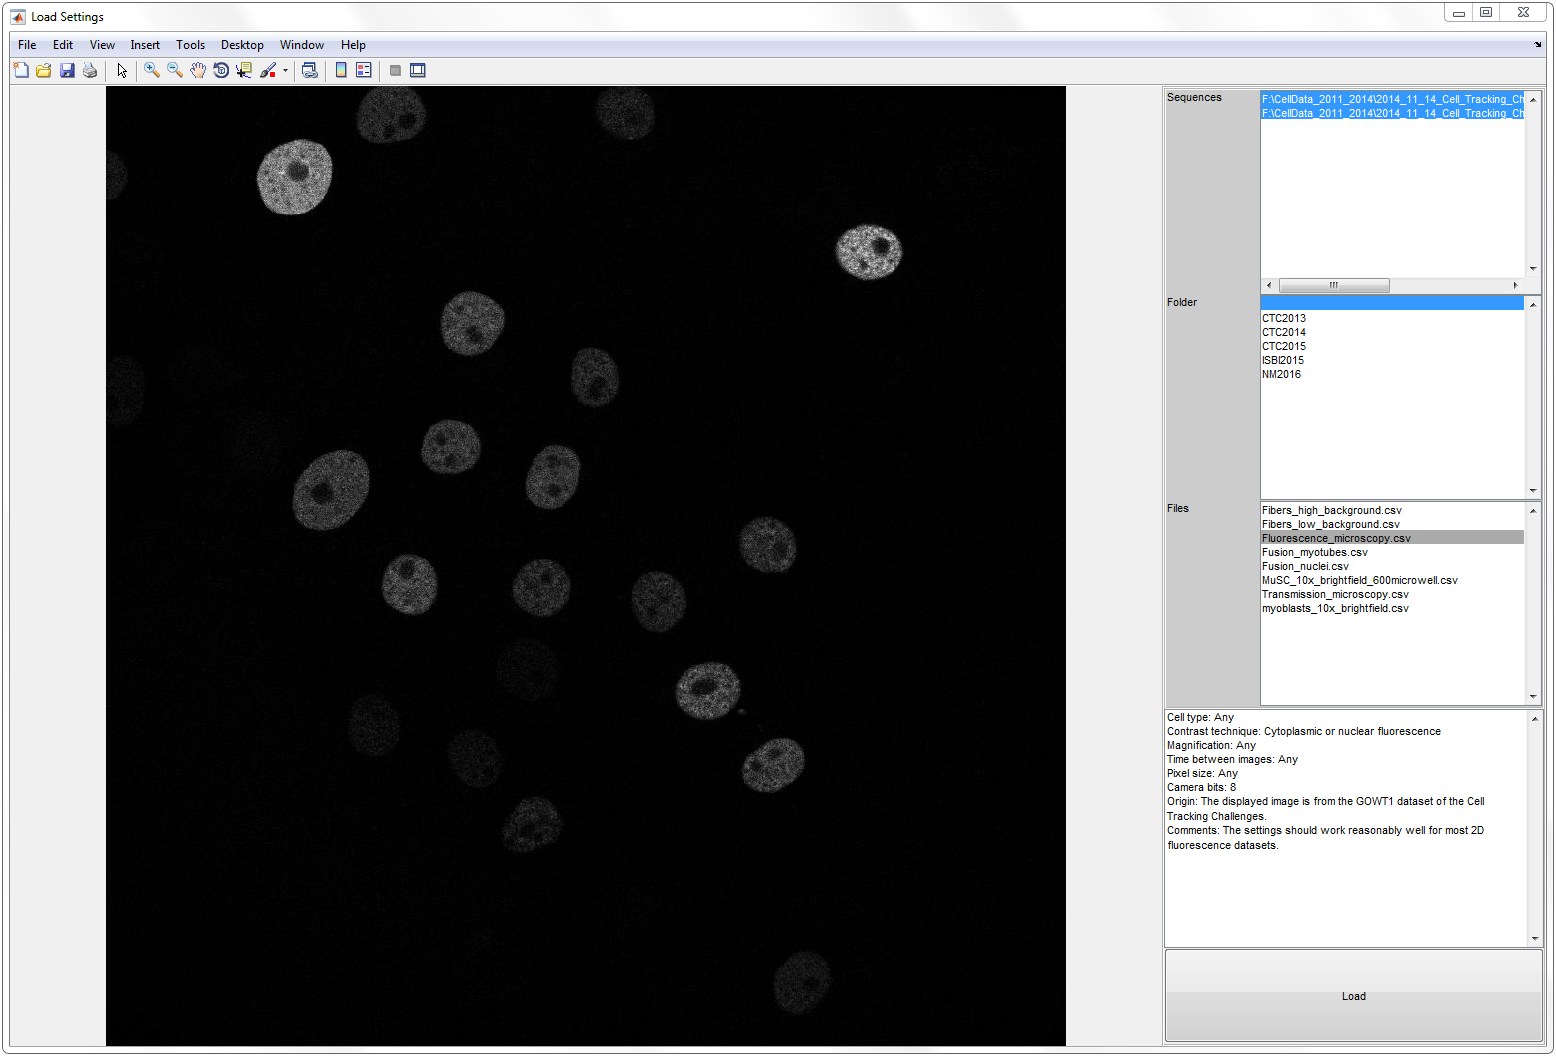
\includegraphics[width = \columnwidth]{figures/loadSettings}
\caption{GUI where you can load settings files.}
\label{fig:load-settings}
\end{center}
\end{figure}

When you have selected a settings file to load, you can choose to load all of the settings saved in the file, or a subset of them. If there are settings for multiple image sequences in the saved file, you can choose what image sequence to load settings from. You can either pick one image sequence name for each image sequence that has been selected in the main GUI or choose a single image sequence name, from which settings will be loaded for all of the image sequences selected in the main GUI. When settings are loaded, the previous settings values will be overwritten, so you need to make a copy of the old settings file if you want to be able to go back to it. There are predefined settings files for tracking of cells in transmission microscopy, tracking of cells in fluorescence microscopy, tracking of MuSCs and myoblasts in bright field microscopy and for segmentation of fluorescently stained muscle histology sections.

\subsection{Saving settings}
Settings can be saved by pressing \menu{Settings/\allowbreak Save Settings}. This will save settings only for the image sequences that have been selected in the main GUI.

\subsection{Settings GUI}
The settings can be modified in the GUI shown in Figure \ref{fig:settings-GUI} by pressing \menu{Settings/\allowbreak Settings}. The settings are grouped into the four categories ''image'', ''segmentation'', ''tracking'', and ''analysis'', which can be selected in the \menu{Category} menu. The image category contains settings which tell the program in what format the images have been saved and how they should be displayed. The segmentation settings tell the program how to find the outlines of the cells, and the tracking settings tell the program how to link the outlines into tracks. The analysis settings describe how the final tracking results should be visualized and analyzed. Many of the settings are binary and take the values 1 or 0 indicating ''on'' or ''off'' respectively. All algorithm parameters are given in pixels and frames. Settings which have no effect at the moment are not displayed, and therefore some settings may appear or disappear when the values for other settings are changed.

\begin{figure}[!htb]
\begin{center}
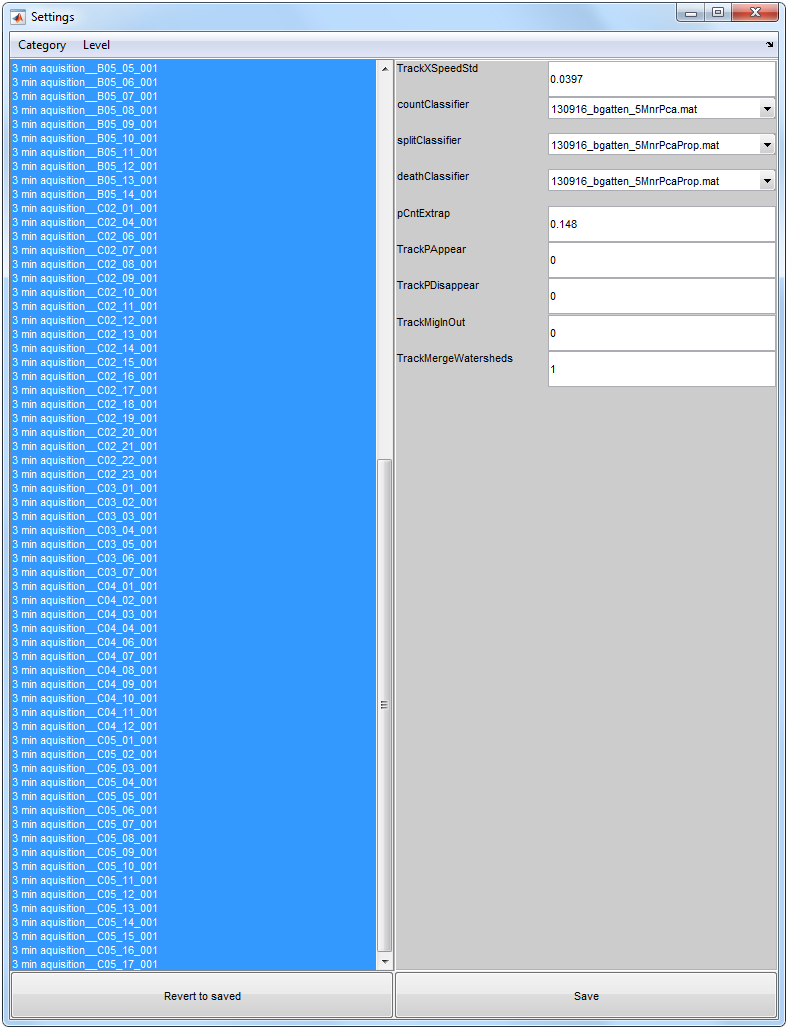
\includegraphics[width = 0.5\columnwidth]{figures/settingsGUI}
\caption{GUI where you can change settings associated with the image sequences.}
\label{fig:settings-GUI}
\end{center}
\end{figure}

\subsection{Image settings}
The settings in the image category are explained in Table \ref{tab:image-settings}. On the basic level, you can only change the number of image bits used by the camera. To access the other settings, you need to select the advanced level. The advanced settings need to be specified correctly in order for 3D data and data with multiple channels to display properly.

\begin{table}[!htb]
\caption{Settings associated with the image files.}
\label{tab:image-settings}
\begin{tabularx}{\textwidth}{lX}
\hline
use & If this setting is 0, the image sequence will not be processed or included in any analysis. \\[5pt] \hline

minWellR & Lower bound in the interval of possible microwell radii in pixels. Set this to \setting{nan} if there are no circular microwells. \\[5pt] \hline

maxWellR & Upper bound in the interval of possible microwell radii in pixels. Set this to \setting{nan} if there are no circular microwells. \\[5pt] \hline

channelNames & Names of the imaged channels, such as \setting{bright field} or \setting{GFP}, separated by \setting{:}. \\[5pt] \hline

channelTags & Unique identifiers, such as \setting{c01} and \setting{c02}, for files belonging to the different channels, separated by \setting{:}. \\[5pt] \hline

sequenceLength & The maximum number of images that will be analyzed in the image sequence. If this setting is left empty, all images are analyzed. \\[5pt] \hline

numZ & The number of $z$-planes in 3D data. This should be 1 for 2D data. \\[5pt] \hline

zStacked & Set this parameter to 1 if the files are tif-stacks with multiple $z$-planes in each file. \\[5pt] \hline

bits & The number of bits used by the camera. If the images have 8 bits, the number of camera bits is almost always 8, but if the images have 16 bits, the camera will often only use 10, 12, or 14 of them. \\[5pt] \hline

voxelHeight & The ratio between the voxel height and the voxel width in 3D data. The value is not used for 2D data. \\[5pt] \hline
\end{tabularx}
\end{table}

\subsection{Fluorescence settings}
\label{sec:settings-fluorescence}
If the data contains multiple channels, you have to tell the program what the channels should be called and how images from the different channels should be identified. The names of the channels should be entered as text strings separated by \setting{:} in the field \setting{channelNames}, and character sequences that are specific to images from the different channels should be entered as text strings separated by \setting{:} in the field \setting{channelTags}. If for example there is a bright field channel and a Green Fluorescent Protein (GFP) channel, the file names of which end with \setting{c01} and \setting{c02} respectively, you can enter \setting{bright field:GFP} into \setting{channelNames} and \setting{c01:c02} into \setting{channelTags}.

\subsubsection{Specifying channel colors}
Once you have entered the names and the tags of the channels correctly, you can specify the colors for the different channels by clicking on \menu{Settings/\allowbreak Set fluorescence display}. That opens the GUI shown in Figure \ref{fig:fluorescence-GUI}, where you can specify colors and ranges of fluorescence values in the different channels.

\begin{figure}[!htb]
\begin{center}
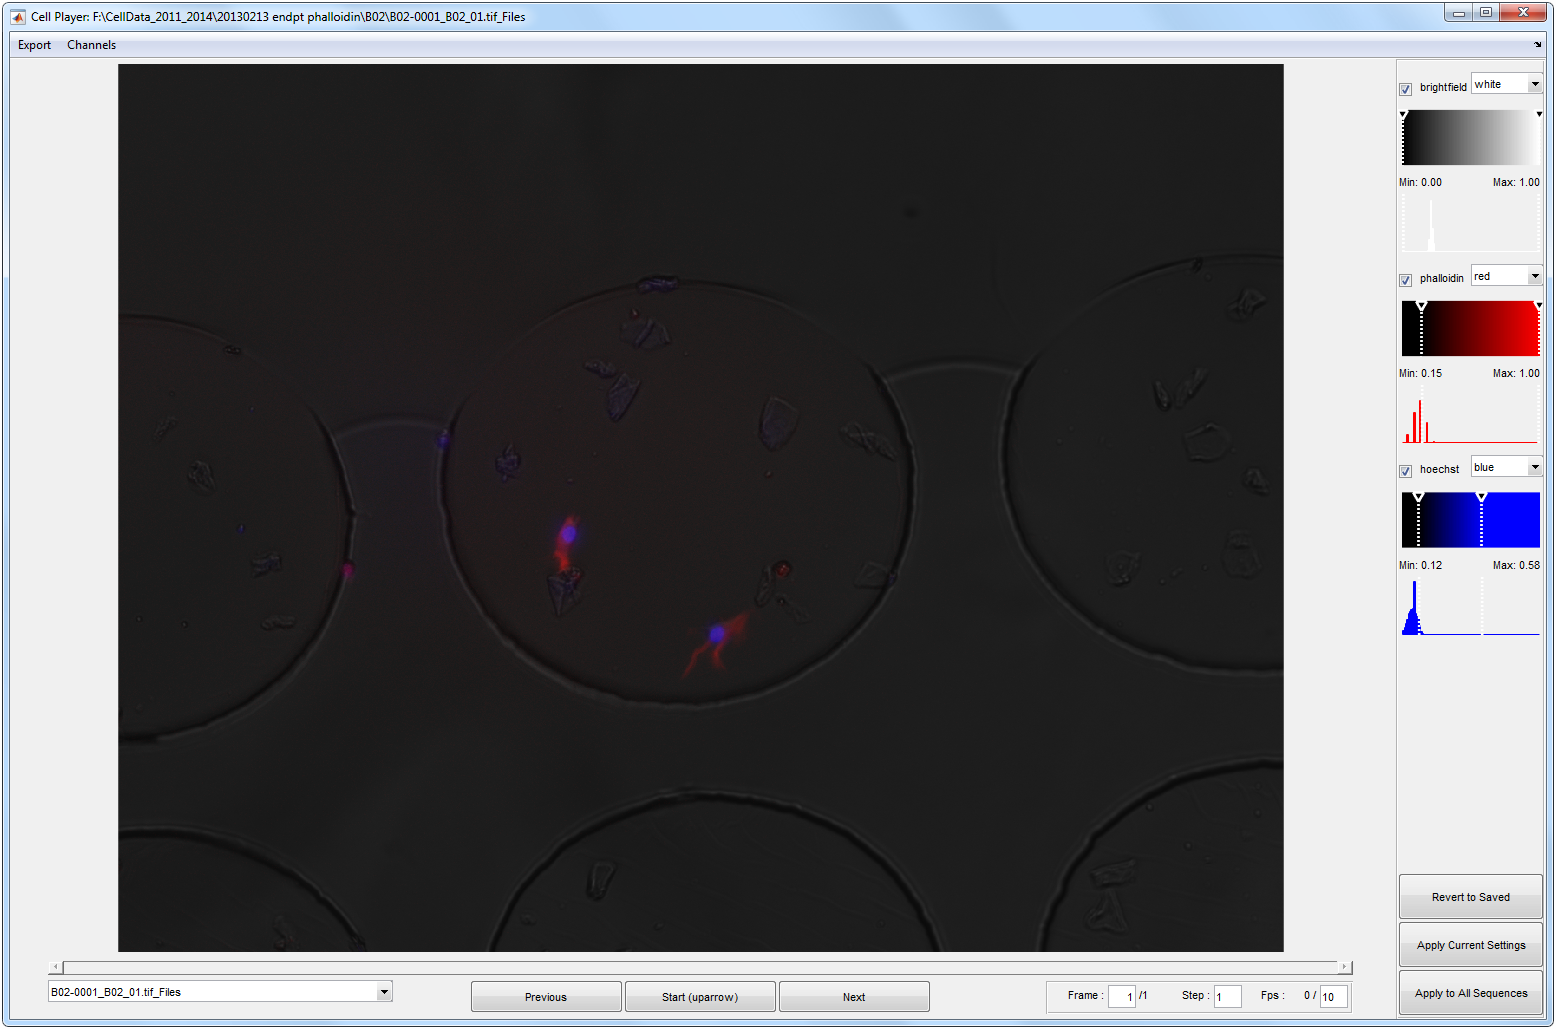
\includegraphics[width = \columnwidth]{figures/fluorescenceGUI}
\credit{Ermelinda Porpiglia, Stanford University}
\caption{GUI where the colors and ranges for different fluorescence channels can be specified.}
\label{fig:fluorescence-GUI}
\end{center}
\end{figure}

\section{Stabilization}
\label{sec:stabilization}
Image stabilization removes camera shake, caused by movements of the stage, by aligning the images in an image sequence. Image stabilization is performed by pressing \menu{Automated/\allowbreak Stabilize}. This brings up a GUI where you can specify the path for the stabilized experiment, and specify how many image sequences should be stabilized in parallel. Performing stabilization creates a new experiment folder with stabilized image sequences, and leaves the original data unaltered. The \control{Queue} button lets you put the stabilization job in a queue, as described in Section \ref{sec:queue}. The image sequences are aligned using a MATLAB implementation of the image stabilization plugin for ImageJ \cite{Li08Stabilizer}. The MATLAB code is less advanced than the ImageJ plugin in that it can only correct for translations in the $x$- and $y$-dimensions. It does however have a few additional features, such as the option to crop the field of view so that no unknown pixel values are included. The implementation has GPU support and will run about 3 times faster if the computer has a GPU.

\section{Cutting of microwells}
Clicking \menu{Automated/\allowbreak Cut microwells} brings up a GUI which cuts out circular microwells from all images in the image sequences and saves the cropped images in a new experiment folder. As for stabilization, you can specify the path for the new experiment, and how many image sequences should be cut in parallel. The original data is unaltered. When both stabilization and cutting is performed, it is best to perform stabilization first, as pixels are lost around the image borders in the stabilization step. The \control{Queue} button lets you put the cutting job in a queue, as described in Section \ref{sec:queue}.

\section{Segmentation}
The first step in analyzing a dataset is to specify a segmentation algorithm that can find the cells in the images, and settings for that segmentation algorithm. Clicking on \menu{Settings/\allowbreak Set segmentation parameters} opens the user interface shown in Figure \ref{fig:segmentation-GUI}, where the cell segmentation is displayed next to a control panel where the segmentation settings can be adjusted. There are many different segmentation algorithms to choose from and the most important ones are described in Section \ref{sec:segmentation-algorithms}. In addition to the segmentation algorithms, you can select preprocessing algorithms that will be applied before the segmentation, and post-processing algorithms that will be applied after the segmentation. These algorithms are independent of the segmentation algorithm and are described in sections \ref{sec:segmentation-preprocessing} and \ref{sec:segmentation-post-processing} respectively.

\begin{figure}[!htb]
\begin{center}
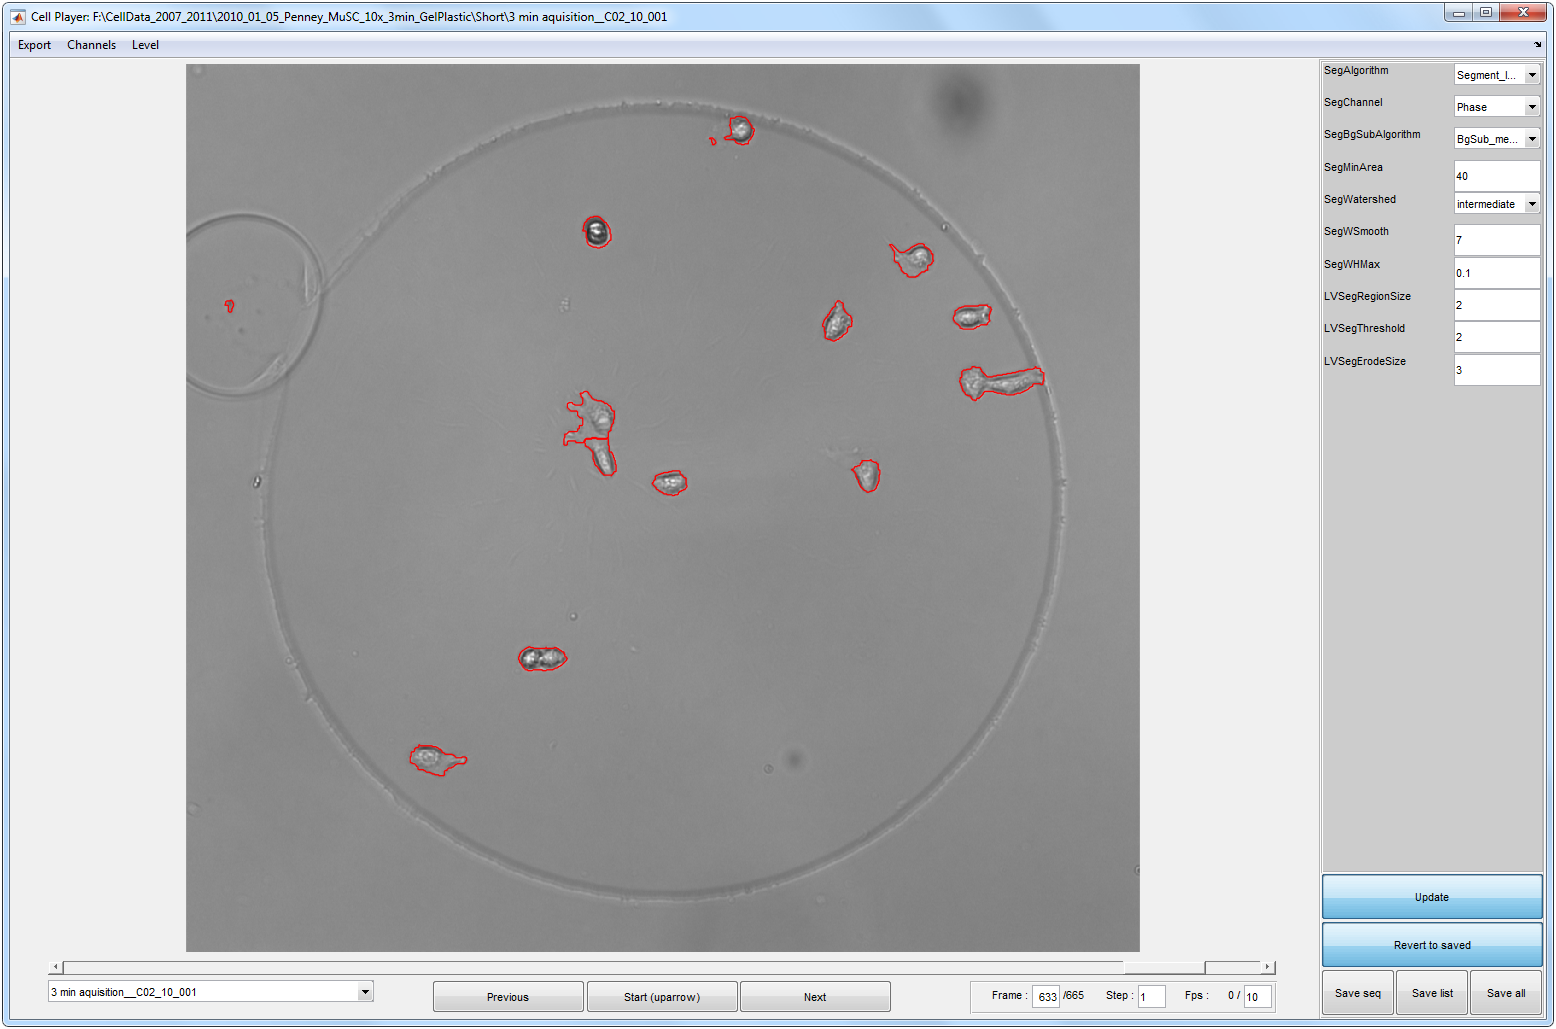
\includegraphics[width = \columnwidth]{figures/segmentationGUI}
\credit{Penney Gilbert, Stanford University}
\caption{GUI where you can set segmentation parameters and preview the segmentation results before you start processing the image sequences.}
\label{fig:segmentation-GUI}
\end{center}
\end{figure}

\subsection{Segmentation GUI}
\label{sec:segmentation-gui}
The GUI has the player structure described in Section \ref{sec:players}, so that different time points and different channels can be displayed easily. It is advisable to look at the segmentation results for multiple image sequences and multiple time points before starting the tracking, to make sure that the selected segmentation settings work for all images. One way to quickly look at multiple time points is to enter \setting{10} into the \control{step} text box in the lower right corner of the interface, to display every 10th image in the sequence, and then play the sequence from beginning to end.

\subsubsection{Choosing a segmentation channel}
Before a segmentation algorithm can be chosen, you must select what channel the segmentation should be applied to, in the dropdown menu \setting{SegChannel}. Channels with nuclear fluorescence are usually easier to segment than channels with cytoplasmic fluorescence which are in turn easier to segment than transmission microscopy channels. Section \ref{sec:settings-fluorescence} has information about how to specify what channels an image sequence has.

\subsubsection{Reusing an old segmentation}
If you are happy with the segmentation in a generated tracking result, you can reuse that segmentation when you rerun the tracking. This can be useful if you have found good segmentation settings but need to change other settings to improve the tracking results. To reuse an old segmentation, you select the name of the corresponding tracking version in the dropdown menu \setting{SegOldVersion} in the segmentation GUI.

\subsubsection{Importing segmentations from other software}
It is possible to generate segmentations using other software (such as CellProfiler or ImageJ) and use them for tracking. To do this, you need to save the segmentations of the individual images as 16-bit tif-files, with label images where the background pixels are 0, the pixels of region 1 are 1, the pixels of region 2 are 2, and so forth. To import the segmentations, you place the label images in a folder with the same name as the image sequence. Then you place the folder in a folder with a name starting with \file{Segmentation}, and place that folder in the \file{Analysis} folder. As an example, the label images could be placed in a folder named \file{[experiment folder]/Analysis/Segmentation\_CellProfiler/[sequence name]}. When you have done this, you can open the segmentation GUI and select the segmentation algorithm \setting{Segment\_import}. There is also a different segmentation algorithm called \setting{Segment\_import\_binary} which converts the label images into binary images. The advantage of this is that you can use post-processing algorithms from the segmentation GUI, and the disadvantage is that it merges adjacent regions. The segmentation algorithms \setting{Segment\_import} and \setting{Segment\_import\_binary} are not shown unless you have a segmentation that can be imported.

In addition to importing a segmentation, you can also import features of segmented regions from CellProfiler. To do this, you need to export the features from CellProfiler to a file called \file{labels.csv}, and put the file in the same folder as the label images. Then the features will be imported together with the segmented regions when you run the tracking. The imported features can currently not be used to train classifiers through the program, but you can write your own MATLAB-scripts to train such classifiers.

\subsubsection{Saving segmentation settings}
To use the segmentation GUI successfully, it is important to understand how segmentation settings are saved to the settings files. The settings that you enter are not automatically saved to the settings files and when you switch to a new image sequence, the settings that you see are not necessarily the settings that have been saved for that file.

The settings that you enter are saved to the settings file first when you press one of the buttons, \control{Save seq}, \control{Save list} or \control{Save all}. \control{Save seq} applies the settings to the currently displayed image sequence, \control{Save list} lets you pick what image sequences the settings should be applied to, and \control{Save all} applies the settings to all image sequences.

When you switch to a new image sequence using either the \control{Previous}-button, the \control{Next}-button, or the image sequence dropdown menu, the settings in the GUI will not be changed unless the \control{Revert to saved}-button is down. Not having the button pressed down lets you verify that a new set of segmentation settings work well on all image sequences in a dataset, without saving it. You can always load the saved settings for the displayed image sequence by pressing the \control{Revert to saved}-button twice.

\subsection{Segmentation algorithms}
\label{sec:segmentation-algorithms}
The user interface has many different segmentation algorithms that can be selected under \setting{SegAlgorithm}. When an algorithm is selected, settings specific to that algorithm will be displayed and settings specific to other algorithms will be hidden. The names of settings specific to a particular segmentation algorithm start with one or multiple letters identifying the segmentation algorithm. In general, \setting{Segment\_localvariance} works well for transmission microscopy images, \setting{Segment\_bandpass}/\setting{Segment\_bandpass3D} works well for fluorescence microscopy images, and \setting{Segment\_fibers} works well for tissue sections with a staining on the cell membranes. The following sub-sections describe the most commonly used segmentation algorithms in detail.

\subsubsection{Segment\_threshold/Segment\_threshold3D}
Thresholding is a simple segmentation algorithm which assumes that the objects of interest are brighter (or darker) than the background. The algorithm creates regions by first labeling all pixels with an intensity above (or below) a threshold as foreground pixels and then computing the connected components of the foreground pixels. This algorithm can work well on fluorescence microscopy images, but usually requires Gaussian smoothing, which is described in Section \ref{sec:smoothing}. The algorithm \setting{Segment\_threshold} is used for 2D data and \setting{Segment\_threshold3D} is used for 3D data, but mathematically the two algorithms are equivalent.

\subsubsection{Segment\_localvariance}
Local variance segmentation computes the sample variance of the pixel intensities in a small region around every pixel. The resulting local variance image is then thresholded to produce a segmentation. The algorithm relies on having a background with a relatively uniform intensity. The algorithm can handle transmission microscopy images created using bright field microscopy, phase contrast microscopy and differential interference contrast (DIC) microscopy. It can also handle fluorescence microscopy and other microscopy techniques where the cells are brighter than the background, but bandpass filtering is likely to work better for such images. Table \ref{tab:local-variance-settings} explains the settings associated with local variance segmentation. The algorithm can detect parts of cells with very low contrast, such as filopodia and lamellipodia but it has problems separating cells in clusters.

\begin{table}[!htb]
\caption{Settings associated with local variance segmentation.}
\label{tab:local-variance-settings}
\begin{tabularx}{\textwidth}{lX}
\hline
LVSegRegionSize & Radius of the region around each pixel, in which the sample variance is computed. \\[5pt] \hline
LVSegThreshold & Threshold applied to the sample variance. Before thresholding, the sample variance is rescaled using the function $f(x) = \log(x+1)$ to give values in a range from 1 to about 5. \\[5pt] \hline
LVSegErodeSize & The number of pixels that will be removed around the borders of all regions using erosion. \\[5pt] \hline
LVSegRegionShape & The shape of the region in which the sample variance will be computed. The available options are \setting{square},  \setting{round}, and \setting{gaussian}. \setting{square} is fastest and usually works well. \setting{gaussian} gives the smoothest borders for large regions. The option \setting{gaussian} puts larger weights on pixels close to the center of the region than pixels further away in the computation of the sample variance. \\[5pt] \hline
LVSegErodeShape & The shape of the structuring element used for erosion. The available options are \setting{square} and \setting{round}. \\[5pt] \hline
\end{tabularx}
\end{table}

\subsubsection{Segment\_bandpass/Segment\_bandpass3D}
Bandpass filtering will usually work well for images where the cells are consistently brighter than the background. It works well for fluorescence microscopy but also for some transmission microscopy techniques such as dark field microscopy and oblique illumination microscopy. The algorithm applies a bandpass filter to the spatial frequencies of the images. This will reduce noise by removing the high frequencies and reduce non-uniform illumination by removing low frequencies. To perform the bandpass filtering, the algorithm first computes a smoothed image $I_{LP_1}$ by convolving the original image with a Gaussian kernel with a small standard deviation. Then a background image $I_{LP_2}$ is created by convolving the image with a Gaussian kernel with a larger standard deviation. The bandpass filtered image is then computed as
\begin{equation}
I_{BP} = I_{LP_1} - \alpha I_{LP_2}.
\label{eq:bandpass}
\end{equation}
Here, $\alpha$ is a free parameter which adds more flexibility. Setting $\alpha=1$ results in a true bandpass filter. The algorithm \setting{Segment\_bandpass} is used for 2D data and \setting{Segment\_bandpass3D} is used for 3D data, but mathematically the two algorithms are equivalent.

Compared to thresholding, bandpass filtering performs better on images with non-uniform illumination, large intensity variations between objects, and objects that form clusters. The only weakness of bandpass filtering that thresholding does not have is that parts of very dim objects that are close to bright objects can disappear from the segmentation. Table \ref{tab:bandpass-settings} explains the settings associated with bandpass segmentation.

\begin{table}[!htb]
\caption{Settings associated with bandpass segmentation.}
\label{tab:bandpass-settings}
\begin{tabularx}{\textwidth}{lX}
\hline
BPSegHighStd & The standard deviation of the Gaussian kernel used to create the background image $I_{LP_2}$. A larger value results in a more blurred $I_{LP_2}$. The value is in pixels and is usually set between 5 and 1000. \\[5pt] \hline
BPSegLowStd & The standard deviation of the Gaussian kernel used to remove noise. Increasing the value removes more noise but also blurs the image. The value is in pixels and is usually set between 1 and 5. The value has to be less than BPSegHighStd. \\[5pt] \hline
BPSegBgFactor & $\alpha$ in Equation \eqref{eq:bandpass}. \\[5pt] \hline
BPSegThreshold & Threshold applied to the bandpass filtered image. The value is usually set between 0.1 and 0.0001. \\[5pt] \hline
\end{tabularx}
\end{table}

\subsubsection{Segment\_fibers}
\label{sec:segmentation-fibers}
Segmentation of muscle fibers is done by applying a watershed transform to a staining of the cell membranes and then merging regions where the intensity on the border between the regions is low compared to the average intensities inside the regions. Table \ref{tab:fiber-settings} explains the three most important settings associated with this segmentation algorithm. There are several other settings, but they are usually less important for the performance. Make sure that \setting{SegChannel} is set to the channel containing the membrane staining.

\begin{table}[!htb]
\caption{Settings associated with segmentation of fibers.}
\label{tab:fiber-settings}
\begin{tabularx}{\textwidth}{lX}
\hline
FibSegBgThreshold & Intensity threshold below which pixels are considered to belong to the background. \\[5pt] \hline
FibSegMergeThreshold & Intensity ratio threshold for merging of adjacent regions. Increasing this value will merge more regions. \\[5pt] \hline
FibSegShapeHMin & The segmented regions are broken into smaller regions using a watershed transform applied to the distance image of the segmentation mask. This parameter specifies the $h$-value of an $h$-min transform applied to the distance image before the watershed transform is computed. Higher values result in fewer region breaks. \\[5pt] \hline
\end{tabularx}
\end{table}

\subsection{Preprocessing}
\label{sec:segmentation-preprocessing}
Sometimes, the images need to be preprocessed before the segmentation algorithms can be applied. This usually means removing a static background using background subtraction or applying smoothing to reduce noise. The image stabilization described in Section \ref{sec:stabilization} is also a type of preprocessing, but the stabilization cannot be previewed in this GUI. If you want to segment cells in microwells, imaged using transmission microscopy and a moving stage, you need to stabilize the image sequence before you can see what the segmentation will be like. You can still get an idea about the segmentation performance from the un-stabilized image sequence, but the background subtraction algorithms described in Section \ref{sec:bgsub} work very poorly without stabilization.

\subsubsection{Background subtraction}
\label{sec:bgsub}
If there are prominent background features, such as the outline of a microwell, it is often necessary to perform background subtraction before the image can be segmented. The most commonly used background subtraction algorithm is called \setting{BgSub\_median}. This algorithm creates a background image by computing a median image over the time dimension of the image sequence, and then subtracts this background image from the individual images of the image sequence. Once the background has been subtracted, regions with a lot of background, such as the microwell, can be attenuated. This will remove artifacts caused by media changes or movements in hydrogel substrates. The amount of attenuation can be specified using the setting \setting{BgSubAtten}. Increasing \setting{BgSubAtten} will remove more background residue, but it can also remove cells or parts of cells from the segmentation. The background subtraction can be visualized by selecting \setting{bgSub} in the \setting{Display} dropdown menu. Figure \ref{fig:MuSC-bgsub} shows an example where a circular microwell has been removed using background subtraction.

\begin{figure}[!htb]
\begin{center}
\credit{Penney Gilbert, Stanford University}\\
\subfloat[][]{\label{subfig:MuSC}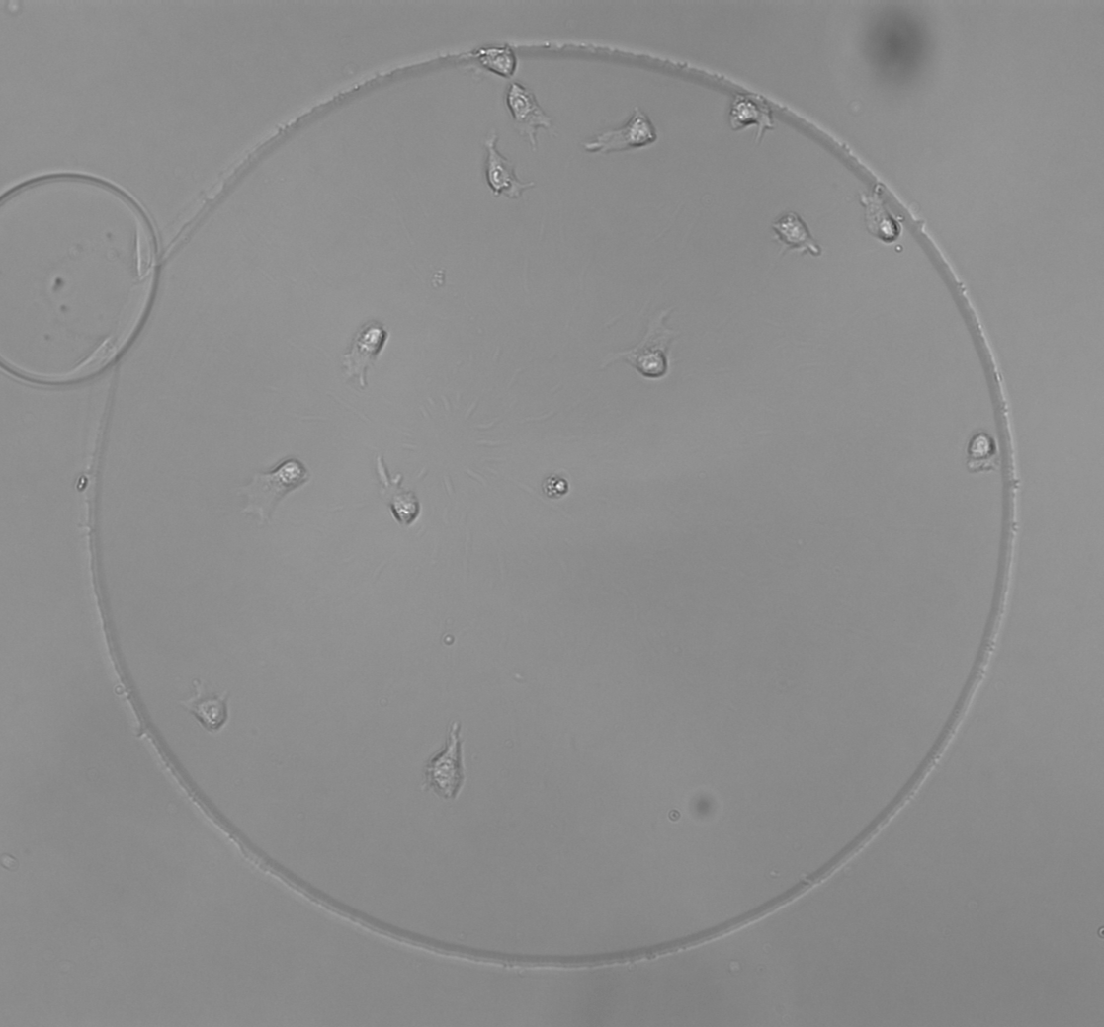
\includegraphics[width=0.45\columnwidth]{figures/MuSC}}
\qquad
\subfloat[][]{\label{subfig:MuSC-bgsub}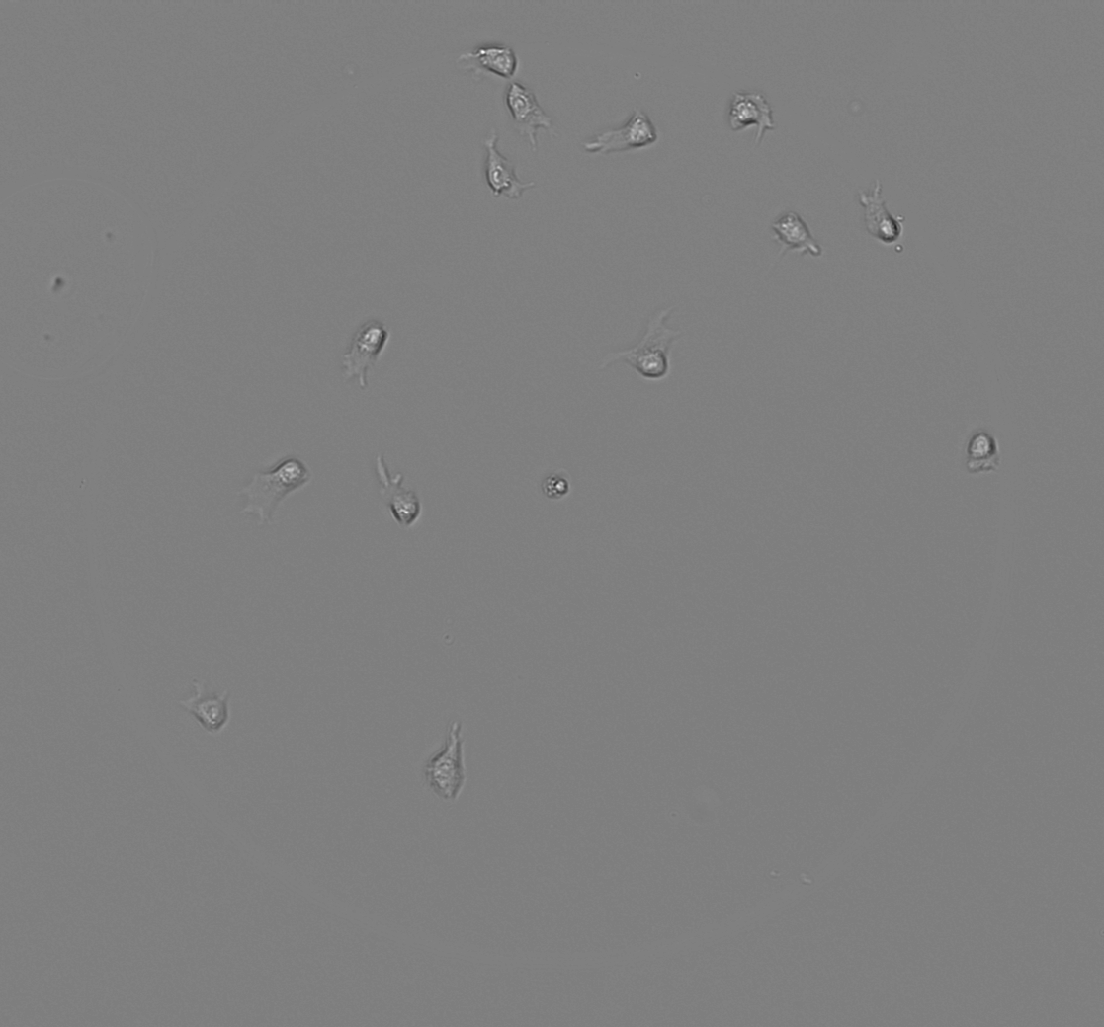
\includegraphics[width=0.45\columnwidth]{figures/MuSC_bgsub}}
\caption{MuSCs in a 600 $\mu$m microwell \protect\subref{subfig:MuSC}, and an image where the microwell has been removed using background subtraction \protect\subref{subfig:MuSC-bgsub}.}
\label{fig:MuSC-bgsub}
\end{center}
\end{figure}

\subsubsection{Smoothing}
\label{sec:smoothing}
The image can be smoothed using a Gaussian kernel, prior to segmentation, by setting \setting{SegSmooth} to a non-zero value, which specifies the standard deviation of the kernel. This is often necessary when threshold segmentation is used, but most other segmentation algorithms have built in mechanisms to handle noise.

\subsection{Light correction}
Setting \setting{SegLightCorrect} to \setting{additive} shifts the intensities of the images so that all images in a sequence get the same mean value. This can be useful if the lighting is not the same throughout the sequence, but otherwise it does not make a big difference.

\subsection{Post-processing}
\label{sec:segmentation-post-processing}
After a segmentation algorithm has been applied, the segmentation can be refined using different post-processing methods. Table \ref{tab:segmentation-post-processing} describes the different settings that are available, and Section \ref{sec:watersheds} explains how watershed transforms can be used to separate cells in clusters.

\LTXtable{\textwidth}{postSegmentationTable.tex}

\subsubsection{Watersheds}
\label{sec:watersheds}
Most segmentation algorithms have problems separating cells in clusters into separate regions. One way of overcoming this problem is to apply a watershed transform to some property of the image which has low values in the middle of cells and high values at the cell borders and in the background. The watershed transform will treat the image as a landscape and simulate flooding of the landscape with water. As the water level rises, lakes will form and the surfaces of the lakes correspond to separated cell regions.

\begin{figure}[!htb]
\begin{center}
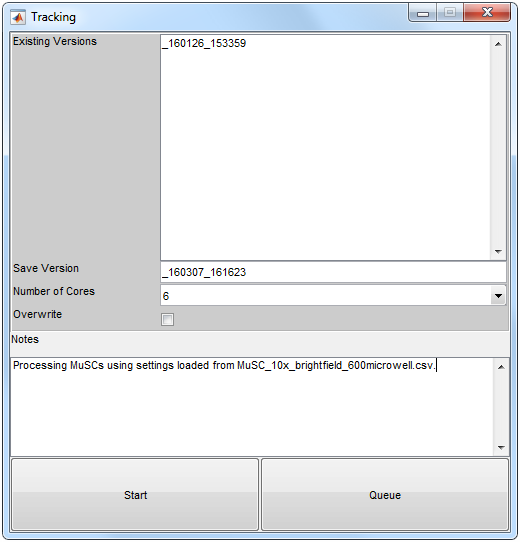
\includegraphics[width = 0.5\columnwidth]{figures/trackingGUI}
\caption{GUI for automated optimization of segmentation parameters.}
\label{fig:segmentation-optimization-GUI}
\end{center}
\end{figure}

\subsection{Automated segmentation optimization}
It is usually hard to find optimal segmentation parameters through manual tweaking. Therefore the BA has a GUI for automated optimization of segmentation parameters. To perform the optimization, you need to export a segmentation ground truth as described in Section \ref{sec:CTC-format}. Then you click on \menu{Settings/Optimize segmentation parameters}, to open the GUI shown in Figure \ref{fig:segmentation-optimization-GUI}. The options in the GUI are explained in Table \ref{tab:segmentation-optimization}.

\begin{table}[!htb]
\caption{Options for segmentation optimization.}
\label{tab:segmentation-optimization}
\begin{tabularx}{\textwidth}{lX}
\hline
Image sequences & Which image sequences to include in the optimization.\\[5pt] \hline

Parameters & Which segmentation parameters to optimize. The segmentation algorithm is selected in the GUI described in Section \ref{sec:segmentation-gui}. \\[5pt] \hline

Scoring function & The scoring function to optimize. \\[5pt] \hline

Optimize individually & If this checkbox is checked, the segmentation parameters are optimized individually for all image sequences. Otherwise, they are optimized jointly. \\[5pt] \hline

Number of iterations & The number of times the optimization algorithm will cycle through all segmentation parameters. \\[5pt] \hline

Maximum number of images & The optimization will include at most this many images from each image sequence in the optimization. This setting can be used to reduce the run time of the optimization. The algorithm will use all images with a segmentation ground truth if the parameter is set to NaN. \\[5pt] \hline

Images with most cells & This setting is shown only if a maximum number of images is set. If the checkbox is checked, the optimization will use the images with most ground truth regions. Otherwise it will use randomly selected images. \\[5pt] \hline

Optimization path & Folder where intermediate results are saved. \\[5pt] \hline
\end{tabularx}
\end{table}

Automated segmentation optimization is available for the segmentation algorithms Segment\_localvariance, Segment\_bandpass, Segment\_bandpass3D, Segment\_threshold, and Segment\_threshold3D. The optimization algorithm optimizes either the SEG measure or the average of the SEG measure and the TRA measure. Both measures are described in Section \ref{sec:performance-evaluation}. The optimization procedure starts from the parameters specified by the user and uses coordinate ascent to find better parameters. Each time better parameters are found, the parameters are saved to the settings files of all image sequences. The initial step length is 25 \% of the start value for each parameter. When a parameter is changed, the step length is increased by 20 \%. When a parameter cannot be changed to produce a better segmentation, the step length is decreased by 20 \%. The parameters and the corresponding performance values are plotted in a separate window during the optimization. More information about the optimization procedure can be found in \cite{Magnusson16Thesis}.

\section{Tracking}
Pressing \menu{Automated/\allowbreak Track} opens the GUI shown in Figure \ref{fig:tracking-GUI}, where you can perform tracking. The segmentation GUI described in Section \ref{sec:segmentation-gui} only changes the segmentation settings and does not generate any segmentation results. The tracking GUI will first run segmentation on all images in a sequence, and then link the segmented regions into tracks. Segmentation of tissue sections is treated as tracking of tissue regions in an image sequence consisting of a single image.

\begin{figure}[!htb]
\begin{center}
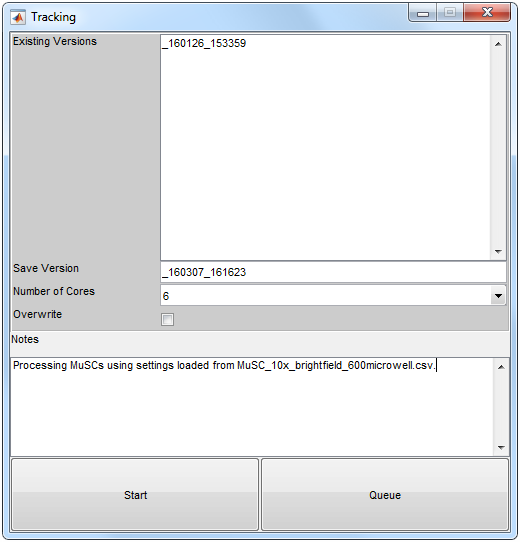
\includegraphics[width = 0.5\columnwidth]{figures/trackingGUI}
\caption{GUI which performs tracking.}
\label{fig:tracking-GUI}
\end{center}
\end{figure}

In the \control{Save Version} text box, you can specify under what name the tracking results should be saved. The default name is the time point when the GUI was opened, in the format \_YYMMDD\_hhmmss, where YY = year, MM = month, DD = day, hh = hour in 24 hour format, mm = minute, and ss = second. The name can be changed to any combination of letters, digits, and underscores, but it can be good to keep the time point as a prefix so that the alphabetical order and the chronological order are the same. The \control{Notes} text box lets you write a short description of the tracking version, where you can describe what settings you used and why. This information is saved in the log file described in Section \ref{sec:tracking-results}. The list box \control{Existing Versions} has a list of all tracking results that have been created previously. If you click on one of them, the corresponding version name and notes will be copied to the appropriate text boxes. That is useful when you want to resume an old processing session.

As for stabilization and cutting, there is a dropdown menu where you can specify how many processor cores should be used for parallel processing. If a single image sequence is tracked, the parallelization is done over time points in the segmentation step. Otherwise, a number of image sequences are processed in parallel, which means that all processing steps are parallelized.

Once the processing of an image sequence has finished, that image sequence will not be processed again if the processing is resumed, even if the settings have been changed. To force the program to redo old computations, you can either specify a new name in \control{Save Version}, or check \control{Overwrite}. Resuming a processing session is described in Section \ref{sec:resume}.

\subsection{Queue}
\label{sec:queue}
Normally, the processing is started by pressing the \control{Start} button, but you can also put the computations in a processing queue by pressing \control{Queue}. This makes it possible to run multiple processing sessions in sequence without having to start all of them separately. This can be useful for example if processing is run overnight or over a weekend.

\subsection{Printouts}
The different processing functions will print progress messages to the command line. When parallel processing is used, progress messages from the different processing threads will be mixed. See section \ref{sec:mac-terminal} for instructions on how to get printouts in the deployed application on Mac.

\subsection{Stopping and restarting}
\label{sec:resume}
You can stop the processing in MATLAB by pressing \command{Ctrl+c}. If the program is busy doing something in a mex-file, it can however take a long time before the execution actually stops. You can resume the processing at a later time by entering the old label in the \control{Save Version} text box. When the processing is resumed, already processed image sequences will not be processed again and the segmentation of partially processed image sequences will be reused. Make sure that \control{Overwrite} is not checked when you want to resume the processing.

\subsection{Track linking settings}
There are a number of settings associated with the track linking. The settings can be changed under \menu{Settings/\allowbreak Settings} and the most important ones are described in Table \ref{tab:tracking-settings}.

\LTXtable{\textwidth}{trackTable.tex}

\subsection{Tracking results}
\label{sec:tracking-results}
All of the tracking results are saved in a folder with the path \file{[Experiment folder]/\allowbreak Analysis/\allowbreak CellData[Save Version]}. The information about the tracks and the outlines of the cells is stored in a mat-file with the same name as the image sequence. The settings that were used are stored in a file named \file{Settings.csv}. Log files with information about the processing that was done are stored in a folder named \file{Logs}. The log files are txt-files named after the image sequences. The files contain notes written by the user, and information about the BA version and the MATLAB version. The folder \file{Compact} contains mat-files with tracking results where cell outlines have been left out. These files are usually much smaller than the files with the complete results. The folder \file{Resume} contains intermediate processing results, primarily segmentation results, that can be used to resume an interrupted processing session. The folder \file{Tracking\_log} contains track linking information which is used only for development and debugging.

For large datasets, such as 3D datasets with hundreds of frames and thousands of cells, the saving of the mat-file can fail due to an out-of-memory error during the compression step. If that happens, the results are instead saved to tif-files using the format described in Section \ref{sec:CTC-format}.

\subsubsection{Exporting tracking results in the CTC format}
\label{sec:CTC-format}
A file format based on tif-images was used in the ISBI Cell Tracking Challenges, which were organized in connection with the International Symposium on Biomedical Imaging in 2013, 2014, and 2015. In the format, label images are saved to 16-bit tif-images, where the background pixels are 0, the pixels of object one are 1, the pixels of object two are 2, and so forth. For 3D datasets, a tif-stack with one slice for each $z$-slice is saved. Additional tracking information is saved in a space separated txt-file with 4 columns. The first column is the track index, the second column is the start frame, the third column is the end frame, and the fourth column is the track index of the parent cell, or 0 if the track does not have a parent. Frame indices are 0-based and track indices are 1-based. The format is described in detail in \cite{Maska14Benchmark, Ortiz15Challenge, Ulman17Objective}.

We have extended the format to incorporate information about death events and false positive regions which are created in the segmentation step but not included in a track in the tracking step. Information about death events are stored in a file named \file{deaths.txt}. This file has two columns. The first column is the track index and the second column is 1 if the track ended in death and 0 otherwise. False positives are saved in a subfolder named \file{false\_positives}. In that folder, information about false positive tracks are saved in the same format as the real cell objects.

The CTC format can be used so save both tracking results, tracking ground truths, and segmentation ground truths. Tracking results and tracking ground truths are saved in the same format, except that the files are named differently. In the segmentation ground truths, 16-bit tif images are used to represent the segmented regions, but there is no track information, and the region numbering goes from 1 to the number of regions in each image. Another difference is that 3D segmentation ground truths can be defined in a single $z$-plane, but this feature is not yet supported by the BA.

The export to the CTC format is performed by selecting the image sequences that the export should be performed for in the main GUI, and then clicking \menu{Export tracks to CTC format/RES tracks}, \menu{Export tracks to CTC format/SEG ground truth}, or \menu{Export tracks to CTC format/TRA ground truth} to export tracking results, segmentation ground truths, or tracking ground truths respectively. Then the user must select an existing tracking result to export. Tracking results are exported to a subfolder named \file{RES/[Image Sequence]\_RES} in the CellData-folder where mat-files with tracking results are normally saved. Ground truths are exported to a folder named \file{[Image sequence]\_GT} in the Analysis folder of the experiment. The tracking ground truth is saved in a subfolder named \file{TRA} and the segmentation ground truth is saved in a subfolder named \file{SEG}. Tracking results can be saved to the CTC format automatically after the tracking step has been executed by setting the option \setting{TrackSaveCTC} to 1 on the advanced level of the tracking settings.

\section{Manual Correction}
\label{sec:manual-correction}
Once the cells have been tracked, the tracks and the outlines of the cells can be visualized and modified in a manual correction interface found under \menu{Manual/\allowbreak Track Correction} and shown in Figure \ref{fig:correction-GUI}. When you open the GUI, no tracking version is selected, so you have to select the desired tracking version in the dropdown menu at the top of the control panel. The outlines of the cells can be visualized independently of the tracks, and the lineage tree can be shown next to the played image sequence. The cells are color coded, so that a cell in the lineage tree can be identified in the image sequence, when the number of cells is small. False positive detections that were found by the segmentation algorithm, but not included in any cell track by the track linking algorithm are shown in white, or a different color specified by the user.

\begin{figure}[!htb]
\begin{center}
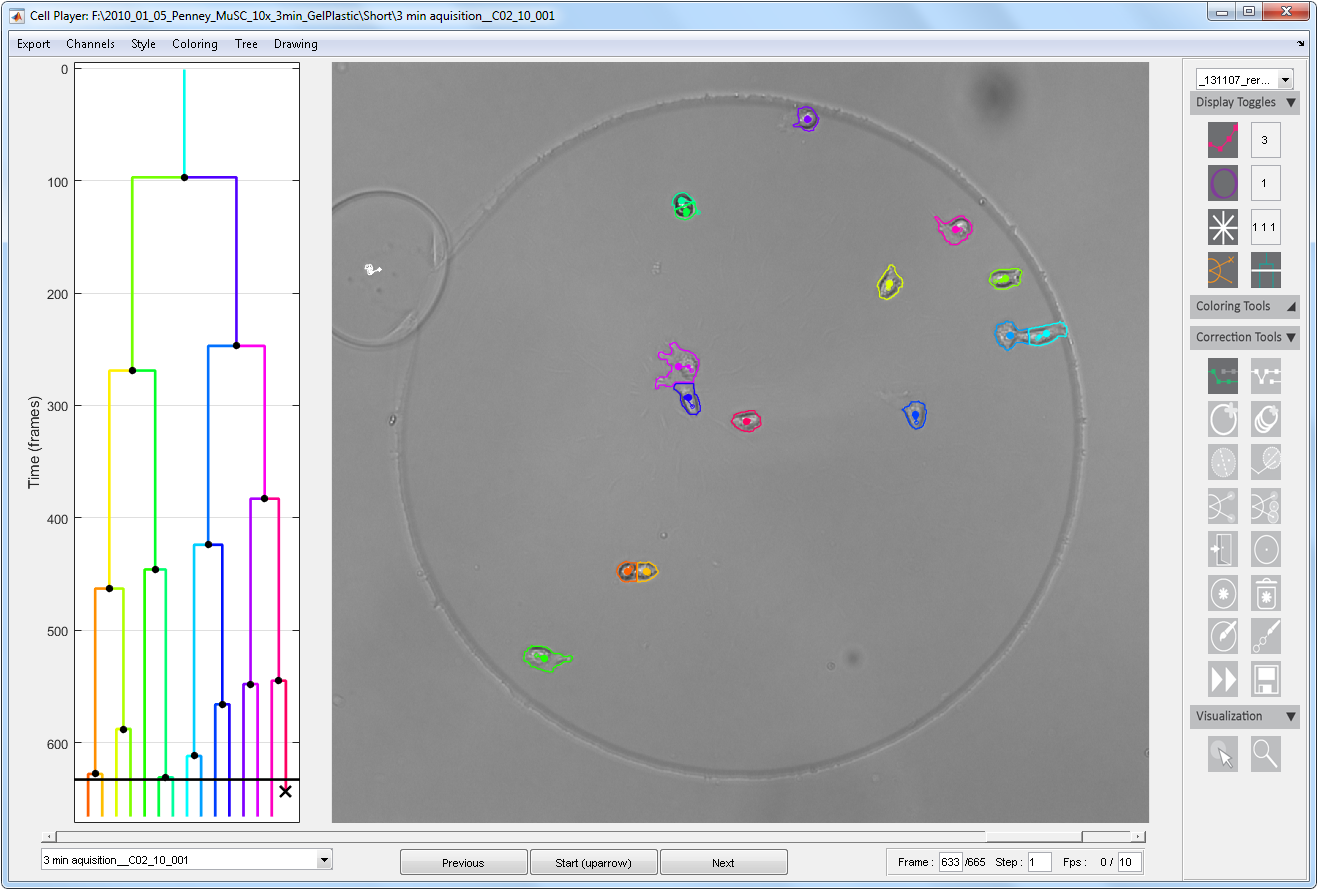
\includegraphics[width = \columnwidth]{figures/correctionGUI}
\credit{Penney Gilbert, Stanford University}
\caption{GUI for visualization and correction of cell tracks and cell outlines.}
\label{fig:correction-GUI}
\end{center}
\end{figure}

The \menu{Style} menu specifies how tracks and outlines should be plotted. The \menu{Default} style is normally used for correction, as is marks cell centroids in the previous and the current image, and as it uses thin lines which do not cover the cells. The \menu{Save} style has thicker lines and visualizes all cell centroids as filled circles. This style is meant to be used when image sequences are recorded. The \menu{ISBI} style uses thin unfilled circles to visualize cell centroids and is therefore suitable for images with small objects that would be covered by filled circles.

The \menu{Coloring} menu has three different coloring alternatives for the cells. The \menu{Rainbow} coloring applies colors from a rainbow to the horizontal axis of the lineage tree. The \menu{Random Hues} coloring gives the cells random colors taken from a rainbow. This alternative is often good during correction, as nearby cells are usually given different colors, and as the colors do not change when the lineage tree is changed due to correction. The \menu{Random Colors} coloring picks random colors from a set of 6 colors.

The controls on the control panel to the right of the image have been grouped into the four groups \control{Display Toggles}, \control{Coloring Tools}, \control{Correction Tools}, and \control{Visualization}. The groups are described in Sections \ref{sec:display-toggles}, \ref{sec:coloring-tools}, \ref{sec:correction-tools}, and \ref{sec:visualization} respectively.

It is important to think about what you want to use the tracking results for. For analysis of cell counts and population averages of parameters like cell size and cell speed, it is usually not necessary to perform correction at all, but for some analysis of individual cells and for analysis of lineage tree parameters, it can be very important to perform correction.

\subsection{Display Toggles}
\label{sec:display-toggles}
The buttons in this group are all toggle buttons which toggle plotting of different types of data on and off. There are also text boxes to specify for how many images back in time tracks and outlines should be plotted. Furthermore, there is a text box where the color of false positive detections can be specified as an RGB triplet.

\subsection{Coloring Tools}
\label{sec:coloring-tools}
The coloring tools let you specify the colors of individual cells. The \control{Change Color of Cell} tool lets you specify a color as an RGB triplet and then click on cells that should have that color. The \control{Change Color of All Cells} tool changes the color of all cells at once.

\subsection{Correction Tools}
\label{sec:correction-tools}
This group contains tools for editing of cell tracks and outlines. Some of the tools perform simple track operations and others speed up the correction of specific tracking errors. Table \ref{tab:track-correction-controls} explains the different tools. The references to large and small circles assumes that the \setting{default} display setting is used. Large filled circles are detections in the current image, small filled circles are detections in the previous image, and small unfilled circles are detections in even earlier images. The segmentation editing tool is described in detail in Section \ref{sec:correcting-outlines}.

\LTXtable{\textwidth}{correctionTable.tex}

\subsubsection{Correcting outlines}
\label{sec:correcting-outlines}
When the \control{Edit/Draw Segments}-button is pressed down, you can modify the outlines of the cells in the current image. The mouse acts as a paint brush when the left mouse button is pressed down and as an eraser when the right button is pressed down. The size of the brush and the eraser can be changed using the scroll wheel on the mouse or using the \control{+} and \control{-} keys on the keyboard.

The \menu{Drawing} menu has several options that affect how outlines are edited. The \menu{Drawing/\allowbreak Create} menu specifies if new regions that are created should become real cells or false positives. The \menu{Drawing/\allowbreak Holes} menu specifies if holes in regions that are drawn should be filled or not. The \menu{Drawing/\allowbreak Merging} menu has three alternatives which specify what should happen if you draw on multiple regions at the same time. With the \menu{Re-break} alternative, the regions that are merged by the drawing will be split between the cells using the $k$-means clustering algorithm used to split regions during the tracking phase. With the \menu{Combine} alternative, the outline of the largest cell is replaced by the union of the drawn region and all blobs that were drawn on. The smaller cells are turned into false positives, and their outlines are removed. With the \menu{Overwrite} alternative, the blob that you started drawing on will be expanded to the drawn region, and take over pixels from other blobs if the pixels are already taken.

\subsubsection{Saving corrected data}
\label{sec:saving-corrected-data}
When either the tracks or the outlines have been edited, the \control{Save}-button can be pressed to save the new cell data. Pressing the \control{Save}-button opens a dialog box where you can specify a name for the new tracking. It is good to add a tag, such as \setting{Corr}, to the corrected tracking versions, to keep track of which versions have been corrected. It is also good to keep the original tracking version, in case it is needed for performance evaluation or some other purpose. Files are overwritten without notifications.

\subsection{Visualization}
\label{sec:visualization}
The \control{Visualization} tool group contains a cell selection tool and a zoom tool. The cell selection tool colors the selected cell orange and all other cells blue. This makes it possible to see where a specific cell has been at earlier time points, and to identify a cell in the lineage tree with a cell in the images. The zoom button enables the zoom tools and the 3D slice selection tools which are always enabled in other players.

\begin{figure}[!htb]
\begin{center}
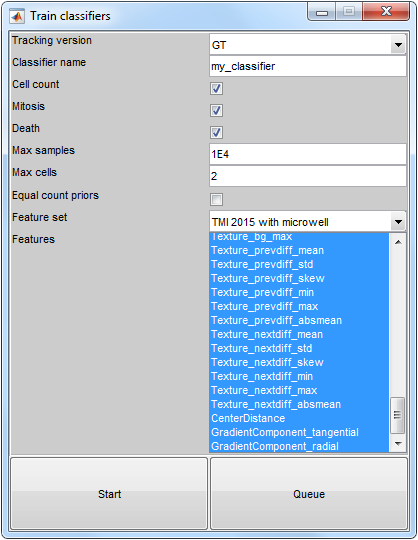
\includegraphics[width = 0.5\columnwidth]{figures/classifierTrainingGUI}
\caption{GUI for training of classifiers.}
\label{fig:classifier-training-GUI}
\end{center}
\end{figure}

\section{Training classifiers}
\label{sec:training-classifiers}
The track linking algorithm can use classifiers to estimate how likely different events are to occur in the regions created by the segmentation algorithm. The program has classifiers that estimate the probability of mitosis, apoptosis and different cell counts inside the individual regions. The classifiers have been created specifically for a particular cell type and a particular imaging technique. If the data that is about to be processed is too different from the data that was used to create the classifier, the tracking performance will be poor. If there is no classifier that matches the data to be processed, it is usually best to set \setting{countClassifier}, \setting{splitClassifier}, and \setting{deathClassifier} in Table \ref{tab:tracking-settings} to \setting{none} and instead specify the settings \setting{pCnt0}, \setting{pCnt1}, \setting{pCnt2}, \setting{pSplit}, and \setting{pDeath} appropriately. Once you have one or more image sequences with corrected cell tracks, you can however create your own classifiers by clicking \menu{Settings/\allowbreak Train classifiers}. This opens the GUI shown in Figure \ref{fig:classifier-training-GUI}. The different options in the GUI are explained in Table \ref{tab:classifier-training}. The trained classifiers are based on multinomial logistic regression. Training of classifiers can require large amounts of corrected data, especially when classifiers for mitosis and apoptosis are trained.

\begin{table}[!htb]
\caption{Options for training of classifiers.}
\label{tab:classifier-training}
\begin{tabularx}{\textwidth}{lX}
\hline
Tracking version & Corrected tracking version to use for training. \\[5pt] \hline

Classifier name & Name of the new classifier. The count, mitosis, and death classifiers are given the same name. \\[5pt] \hline

Cell count & Trains a cell count classifier. \\[5pt] \hline

Mitosis &  Trains a mitosis classifier. \\[5pt] \hline

Death &  Trains a cell death classifier. \\[5pt] \hline

Max samples & The maximum number of training examples in each class. Using more training examples usually gives a better classifier, but the training takes longer. There is usually no point in using more than 1E5 training examples. The training examples are drawn randomly if there are more examples than the specified number. In that case, the training examples are weighted in the training, so that the original balance between the classes is maintained. \\[5pt] \hline

Max cells & The maximum number of cells that the cell count classifier can handle in a region. If the setting is 2, the classes of the classifier will be 0 cells, 1 cell, and 2 or more cells. A maximum of 2 is usually good, as there are often too few examples of regions with 3 cells to train a reliable classifier. \\[5pt] \hline

Equal count priors & If this checkbox is checked, the priors of the classes in the cell count classifier will be set equal. This can be good in inhomogeneous datasets where different parts have very different priors. \\[5pt] \hline

Feature set & The set of region features to use for classification. \\[5pt] \hline

Features &  The features in the selected feature set. \\[5pt] \hline
\end{tabularx}
\end{table}

\subsection{Features}
The region features are grouped into feature sets that can be selected in the \control{Feature set} dropdown menu. The feature set ''ISBI 2012'' is taken from \cite{Magnusson12Viterbi} and the feature set ''TMI 2015'' is taken from \cite{Magnusson15Viterbi}. The feature set ''All features'' is the union of all features in ''ISBI 2012'' and ''TMI 2015''. All of these feature sets were designed for tracking of adherent cells in bright field microscopy, but they should work well for other cell types and imaging techniques as well. All of the feature sets have options in the dropdown menu with and without microwells. The only difference is that the feature ''CenterDistance'' has been added to the options with microwells. These options should only be used if you are tracking cells in circular microwells. You can select a subset of the features in a feature set by marking the features you want in the \control{Feature} listbox.

\begin{table}[!htb]
\caption{Settings associated with the analysis of cell tracks.}
\label{tab:analysis-settings}
\begin{tabularx}{\textwidth}{lX}
\hline
condition & The name of the experimental condition for each image sequence. This affects how the image sequences are grouped in the analysis. \\[5pt] \hline

pixelSize & Pixel size of the camera sensor in $\mu$m. The pixels are assumed to be square. \\[5pt] \hline

magnification & The magnification of the camera objective. \\[5pt] \hline

dT & The time in seconds between image sequence frames. \\[5pt] \hline

startT & Time in hours when the imaging was started. The zero time point is usually defined as the time when the cells were plated. \\[5pt] \hline

minPlotT & The first time point (in hours) that should be included in analysis plots. If this is left empty, the plots start with the first image. \\[5pt] \hline

maxPlotT & The last time point (in hours) that should be included in analysis plots. If this is left empty, the plots end  with the last image. \\[5pt] \hline
\end{tabularx}
\end{table}

\section{Analysis}
Once the tracks and outlines of all cells have been computed and possibly corrected, different types of analysis can be performed on the data. The program already has a lot of analysis functions for commonly used readouts, but for more complex and application specific readouts, custom analysis functions can be developed and easily incorporated into the program. Settings associated with analysis are explained in Table \ref{tab:analysis-settings}. To get the right conversions from pixels and frames to micrometers and hours, you need to specify the settings \setting{pixelSize}, \setting{magnification} and \setting{dT}. Otherwise all results will be given in pixels and frames, even if the axis labels and printouts say ''micrometers'' and ''hours''.

\subsection{Cell analysis GUI}
Under \menu{Analysis/\allowbreak Cell Analysis GUI}, you find the GUI shown in Figure \ref{fig:cell-analysis-GUI}, which is used for plotting of parameters of individual cells over time. The plots include data from a particular clone or image sequence and have a curve for each cell. Examples of parameters that can be plotted are axis ratios, lineage trees, cell sizes and the total distance traveled by each cell. The \control{Tracking Version} dropdown menu specifies what tracking version should be used for the analysis. Pressing \control{Start} cycles through the image sequences or the clones and shows a plot for each of them.

\begin{figure}[!htb]
\begin{center}
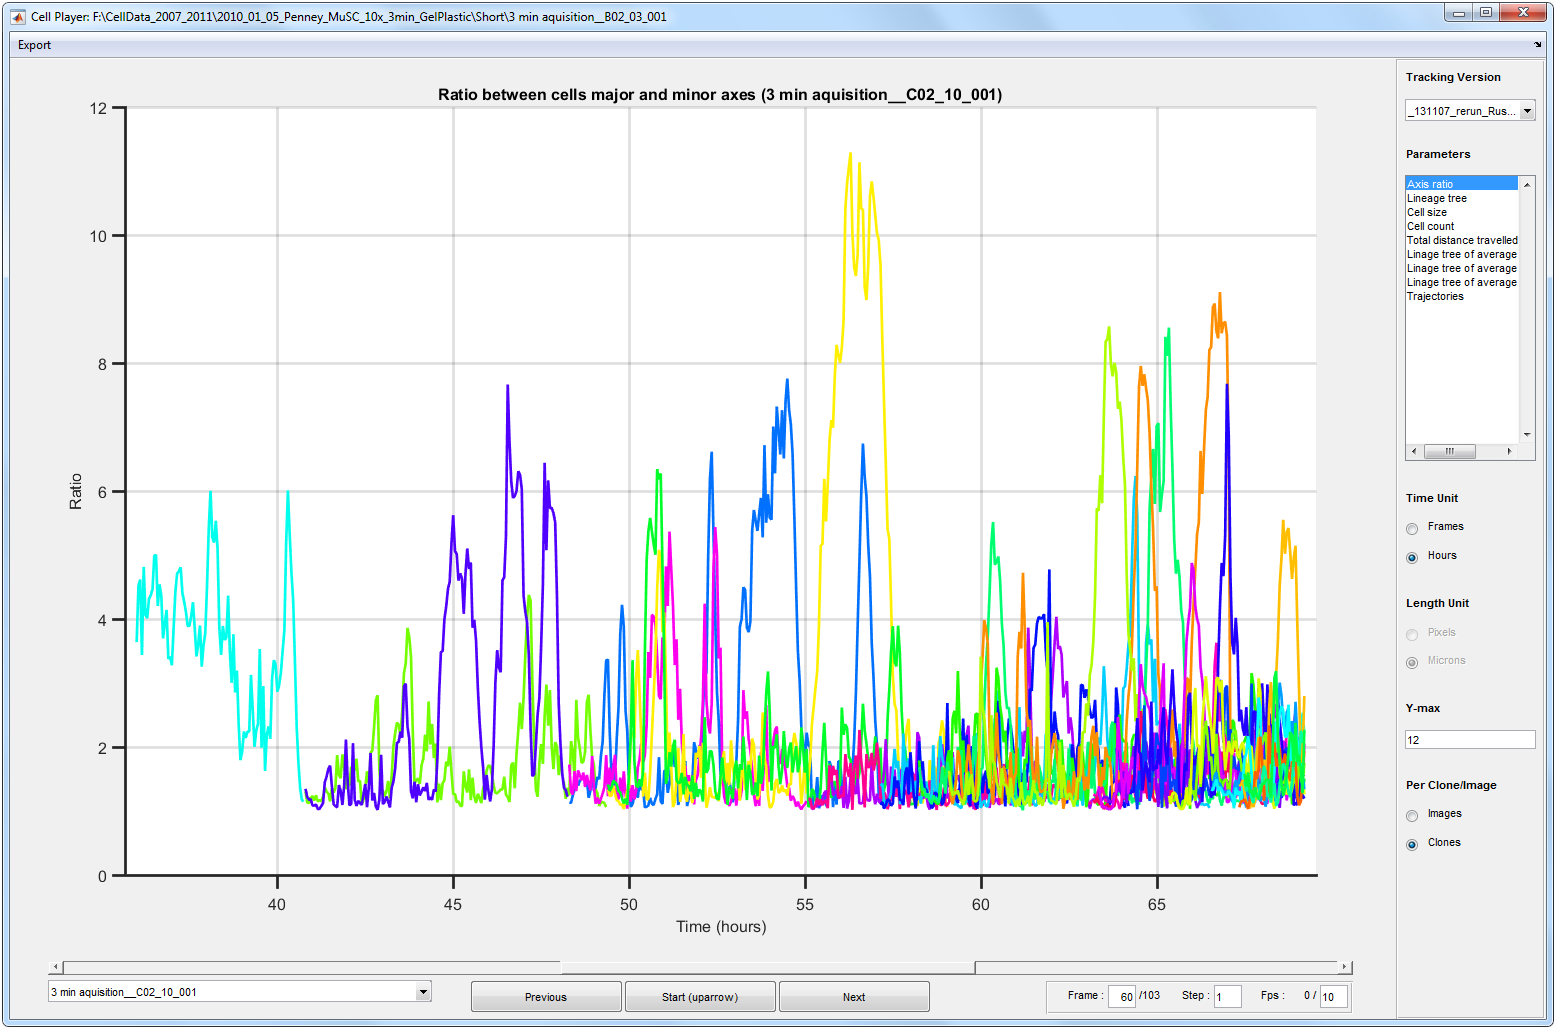
\includegraphics[width = \columnwidth]{figures/cellAnalysisGUI}
\caption{GUI for plotting of parameters of individual cells over time. The displayed plot shows axis ratios of muscle stem cells as a function of time.}
\label{fig:cell-analysis-GUI}
\end{center}
\end{figure}

\subsection{Population analysis GUI}
Under \menu{Analysis/\allowbreak Population Analysis GUI}, you find the GUI shown in Figure \ref{fig:population-analysis-GUI}, which is used for plotting of parameters averaged over the life spans of the cells. Every cell in the dataset will therefore have a value associated with it and the distributions of the values can be compared between different experimental conditions. There are a number of parameters, such as average speed, average axis ratio, and average size, that can be visualized. There are also a number of different plotting methods that can be used for visualization.

\begin{figure}[!htb]
\begin{center}
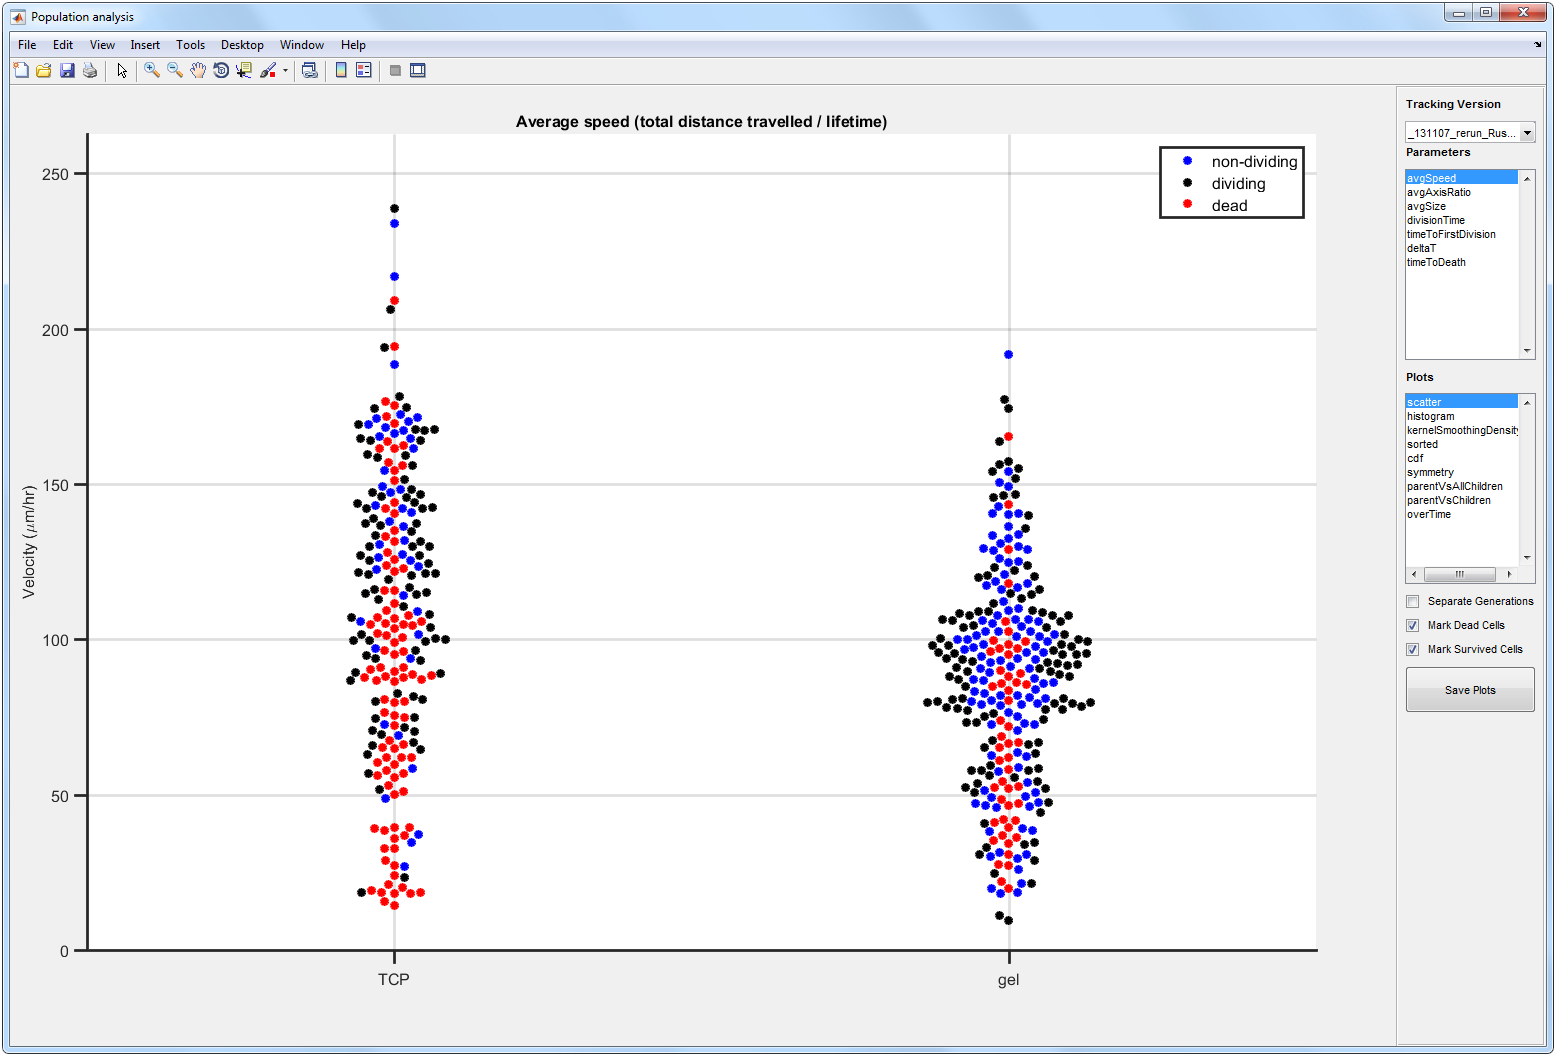
\includegraphics[width = \columnwidth]{figures/populationAnalysisGUI}
\caption{GUI for plotting of parameters averaged over the life spans of cells. The displayed plot shows the average speeds of muscle stem cells.}
\label{fig:population-analysis-GUI}
\end{center}
\end{figure}

\subsection{Scatter Plot Analysis GUI}
While the Population Analysis GUI plots one cell parameter at a time, the Scatter Plot Analysis GUI lets you plot pairs of cell parameters against each other, to see how different parameters are connected. Figure \ref{fig:scatter-plot-GUI} shows the GUI. You can choose what tracking version to analyze, which parameters to plot on the two axes, and how the cells should be colored. If you choose to color the cells by fate, dividing cells are black, non-dividing cells are blue, and dying cells are red. By unchecking the checkboxes ''Mark Dead Cells'' and ''Mark Survived Cells'', you can however color the dying and surviving cells black like the dividing cells.

\begin{figure}[!htb]
\begin{center}
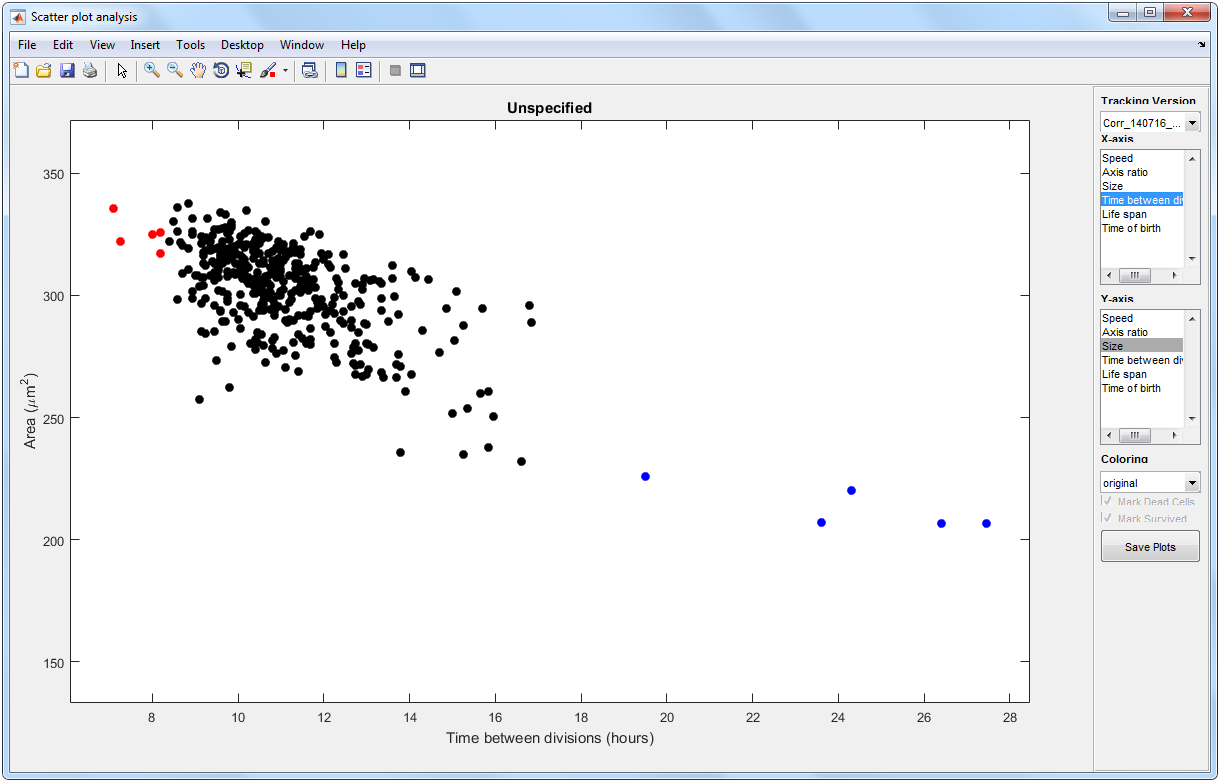
\includegraphics[width = \columnwidth]{figures/scatterPlotGUI}
\caption{GUI where you can plot pairs of cell parameter against each other. The plot shows cell size against the time between divisions for a clone of hematopoietic stem cells. The cells were colored in the manual correction GUI.}
\label{fig:scatter-plot-GUI}
\end{center}
\end{figure}

\subsection{Plot GUI}
Under \menu{Analysis/\allowbreak Plot GUI}, you find the GUI shown in Figure \ref{fig:plot-GUI}, were you can select analysis functions from a list and apply them to all image sequences or a subset of them. While the Cell Analysis GUI and the Population Analysis GUI plot raw parameter values for individual cells, most of the analysis functions in Plot GUI compile the parameter values into plots which quantify different cell behaviours. The tracking results are loaded only once even if multiple functions are executed, and all of the functions operate on the compact tracking results without blob outlines, which load faster than the full tracking results. Therefore, the loading of tracking results is relatively fast. The different parts of the GUI are explained in Table \ref{tab:plot-GUI}.

\begin{figure}[!htb]
\begin{center}
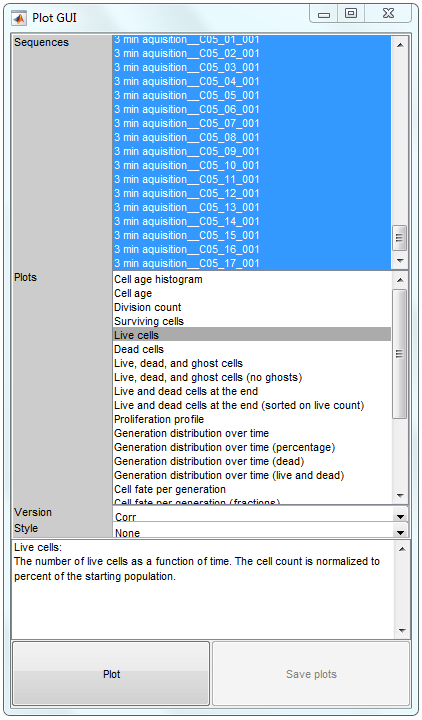
\includegraphics[width = 0.5\columnwidth]{figures/plotGUI}
\caption{GUI where you can apply analysis functions to cells in tracked image sequences.}
\label{fig:plot-GUI}
\end{center}
\end{figure}

\begin{table}[!htb]
\caption{Controls in the Plot GUI.}
\label{tab:plot-GUI}
\begin{tabularx}{\textwidth}{lX}
\hline
Sequences & List where a set of image sequences can be selected for analysis. \\[5pt] \hline

Plots & List where one or more potting functions can be selected for execution. When a plotting function has been selected, a description of the function appears in the text box above the buttons at the bottom of the window. \\[5pt] \hline

Version & The name of the tracking version that will be loaded. \\[5pt] \hline

Style & Plotting style that will be applied to the plots after the analysis functions have been executed. The style ''Screen'' has thin lines, small markers, and a grid, for detailed analysis on a computer screen. The style ''Print'' has thicker lines, larger makers, and larger fonts, for legible printing on a full page. The style ''Publication'' has even thicker lines, larger markers, and larger fonts, for legible figures in a publication. If you do not select a style, you will get whatever comes out of the plotting functions, and that is usually similar to the style ''Print''.\\[5pt] \hline

Plot & Executes all the selected plotting functions on the selected image sequences. \\[5pt] \hline

Save Plots & Once you have run the plotting functions, you can press this button to open a GUI where you can save the plots to files. \\[5pt] \hline
\end{tabularx}
\end{table}

\subsection{Exporting statistics to csv-files}
If you want to perform statistical analysis on the tracking results, without writing your own MATLAB code, you can export data for different cell parameters to csv-files by pressing \menu{Analysis/\allowbreak Statistics}. That will export the mean, standard deviation, median, minimum, and maximum of the cell parameters average speed, average axis ratio, average size, time between divisions, and time to first division. The csv-files will contain tables where the cells are grouped by experimental condition, and other tables where the cells are grouped both by experimental condition and cell generation. The number of cells in each group is also stated, so that you can perform statistical tests. The csv-files can be opened in Excel and in text editors.

\section{Performance evaluation}
\label{sec:performance-evaluation}
In the BA, segmentation performance and tracking performance can be evaluated using the measures SEG and TRA, which were used to score algorithm performance in the ISBI Cell Tracking Challenges. The BA has its own MATLAB implementations of the two measures.

Before the performance evaluation can be performed, a segmentation or tracking ground truth has to be created and exported in the CTC format, as described in Section \ref{sec:CTC-format}. The tracking results to be evaluated are exported automatically to the CTC format if that has not been done already. The performance information is saved to log files in the \file{RES} folders described in Section \ref{sec:CTC-format}, so that it does not need to be recomputed every time the user wants to review the performance. It is however necessary to delete the log files manually if the ground truth files are changed.

\subsection{SEG measure}
The segmentation performance can be evaluated using the SEG measure by clicking \menu{Analysis/SEG Segmentation performance} with advanced menus turned on. The SEG measure computes the average Jaccard index between ground truth regions and matching segmented regions. A segmented region is considered matching if it covers more than 50 \% of the ground truth region. The Jaccard index is the number of pixels in the intersection of the regions divided by the number of pixels in the union of the regions. Ground truth regions with no matching segmented region are given a Jaccard index of 0. An advantage of the performance measure is it is enough if the ground truth contains a representative subset of cells. A disadvantage is that it does not penalize false positives. The measure is described in detail in \cite{Maska14Benchmark, Ortiz15Challenge, Ulman17Objective}.

The SEG measure disfavors segmentation algorithms with severe under-segmentation, as segmented regions are disregarded if they cover 50 \% or less of the ground truth region. To overcome this problem, we provide a relaxed SEG measure which matches each ground truth region to the segmented region which gives the highest possible Jaccard index, without requiring an overlap of more than 50 \%. The relaxed SEG measure is used if the check box named \control{Relaxed SEG measure} is checked. Otherwise, the traditional SEG measure is used.

\subsection{TRA measure}
The track linking performance can be evaluated using the TRA measure by clicking \menu{Analysis/TRA Tracking performance} with advanced menus turned on. The TRA measure is a normalized version of the AOGM measure \cite{Matula15Accuracy}. The AOGM measure is a weighted sum of tracking errors where the weights are taken from Table \ref{tab:TRA-penalties}. The weights are roughly proportional to the time it takes to manually correct errors of the different types. The measure as a whole is therefore a measure of how long it takes to correct the tracking results manually.

\begin{table}
  \centering
  \caption{Penalties for tracking errors in the AOGM measure.}\label{tab:TRA-penalties}
  \begin{tabular}{ll}
    Error & Penalty \\
    \hline
    False negative & 10 \\
    Merged regions & 5 \\
    False positives & 1 \\
    Missing links & 1.5 \\
    Incorrect links & 1 \\
    Links of the wrong type & 1
  \end{tabular}
\end{table}

The TRA measure is computed by normalizing the AOGM measure according to
\begin{equation}
\text{TRA} = 1 - \frac{\min(\text{AOGM},\text{AOGM}_0)}{\text{AOGM}_0},
\end{equation}
where $\text{AOGM}_0$ is the AOGM measure of an empty tracking result. The TRA measure is described in \cite{Ortiz15Challenge, Ulman17Objective}.

\section{Specific types of data}
This section describes methods and settings that can be used for specific types of data that have been processed using the BA in the past. Section \ref{sec:MuSC} is about tracking of muscle stem cells (MuSCs) imaged using bright field microscopy, Section \ref{sec:fibers} is about analysis of fluorescently stained histological sections of muscle fibers, and Section \ref{sec:fusion} is about analysis of myotube fusion assays with fluorescently stained images.

\subsection{MuSCs}
\label{sec:MuSC}
This section describes how to process image sequences of MuSCs, imaged using bright field microscopy. It is assumed that the cells are grown in circular microwells with a radius of approximately 600 $\mu$m and that they are imaged every 3 minutes using 10$\times$ magnification. Figure \ref{fig:MuSC} shows an image from such an image sequence.

\begin{figure}[!htb]
\begin{center}
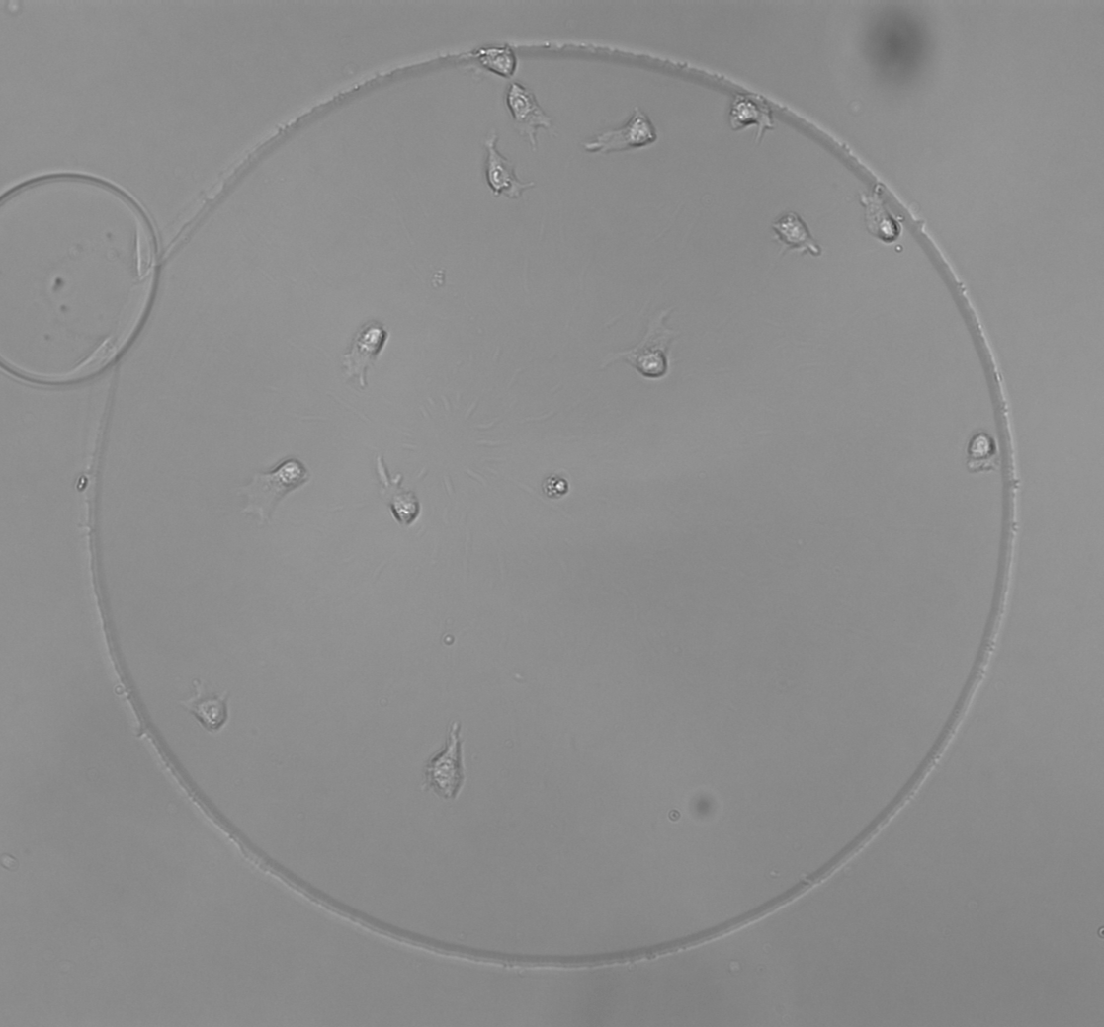
\includegraphics[width = \columnwidth]{figures/MuSC}
\credit{Penney Gilbert, Stanford University}
\caption{MuSCs in a 600 $\mu$m microwell, imaged using 10$\times$ bright field microscopy.}
\label{fig:MuSC}
\end{center}
\end{figure}

To process data of the type described above, you can go to \menu{Settings/\allowbreak Load Settings} and load the file \file{MuSC\_\allowbreak  10x\_\allowbreak brightfield\_\allowbreak 600microwell.csv}, which has settings optimized for this type of data. To process data with an imaging interval of 5 minutes, you should increase \setting{TrackXSpeedStd} in Table \ref{tab:tracking-settings} and \setting{dT} in Table \ref{tab:analysis-settings} by a factor of 5/3. If you want to track cells grown on a flat culture substrate without microwells, you need to change \setting{minWellR} and \setting{maxWellR} in Table \ref{tab:image-settings} to \setting{nan}. The settings for tracking of MuSCs will work well for other cell types imaged using 10$\times$ bright field microscopy as well, as long as the cells look and behave similarly to MuSCs. We have for example tracked myoblasts with good results.

The program will use background subtraction to remove the microwell outline during the segmentation step and therefore it is crucial that you apply image stabilization, as described in Section \ref{sec:stabilization}. Otherwise the segmentation will fail completely. If you changed the culturing media during the experiment, the background subtraction \ref{sec:bgsub} can be problematic. If you find that the segmentation algorithm picks up the microwell boundary, you can try increasing the \setting{BgSubAtten} setting associated with the background subtraction, or increase the \setting{LVSegThreshold} setting associated with the local variance segmentation algorithm. The local variance segmentation algorithm is robust to differences between image sequences, so it should be possible to use the same segmentation settings for all image sequences in an entire experiment.

\subsection{Muscle fibers}
\label{sec:fibers}
This section describes how to process fluorescently stained histological sections of muscle fibers. To segment the fibers, the program requires a staining of laminin or some other protein marking the outlines of the fibers. It does not matter what other channels have been included in the experiment. Figure \ref{fig:fibers} shows an example of a mouse muscle section stained for laminin, GFP and DAPI, that has been analyzed successfully using the program.

\begin{figure}[!htb]
\begin{center}
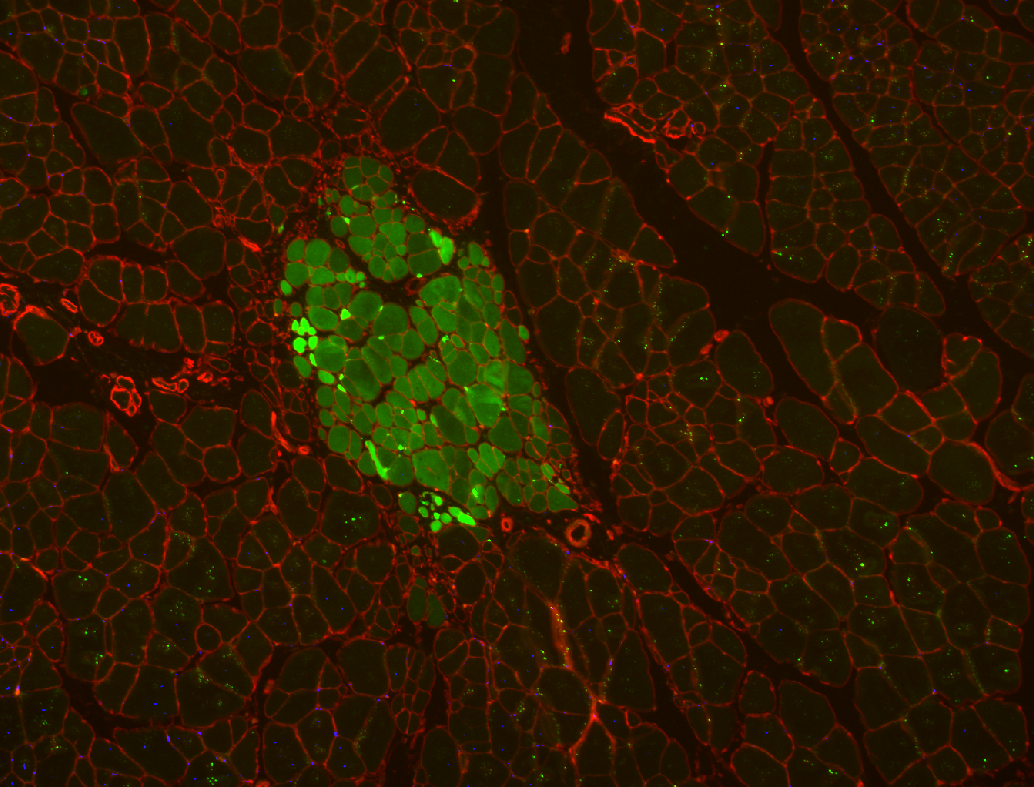
\includegraphics[width = \columnwidth]{figures/fibers}
\credit{Foteini Mourkioti, Stanford University}
\caption{A mouse muscle histology section stained for laminin, GFP and DAPI.}
\label{fig:fibers}
\end{center}
\end{figure}

To analyze muscle sections, you first need to load the appropriate settings by clicking \menu{Settings/\allowbreak Load Settings} and loading either \file{Fibers\_\allowbreak low\_\allowbreak background.csv} or \file{Fibers\_\allowbreak high\_\allowbreak background.csv}. \file{Fibers\_\allowbreak low\_\allowbreak background.csv} is for images with low background, where the cracks between the fibers have low intensity in all imaged channels. If it is hard to distinguish cracks from fibers, based only on pixel intensities, \file{Fibers\_\allowbreak high\_\allowbreak background.csv} should be used. In this case, you may have to remove cracks between fibers, using the manual correction user interface described below, after the images have been processed. Once you have loaded the settings, you will need to specify the settings \setting{channelNames} and \setting{channelTags}, as described in Section \ref{sec:settings-fluorescence}, so that the program knows how to find the channel with the cell membrane staining.

Before you start processing the images, you need to check that the fibers will be segmented correctly, by opening the segmentation GUI described in Section \ref{sec:segmentation-gui}. If you are not happy with the segmentation results, you can try changing the settings \setting{FibSegBgThreshold} and \setting{FibSegMergeThreshold} described in Table \ref{tab:fiber-settings}. Also make sure that the segmentation setting \setting{SegChannel} is set to the channel with the cell membrane staining.

There is a manual correction user interface designed specifically for correction of muscle fiber segmentations. The user interface is similar to that described in Section \ref{sec:manual-correction}, and it is opened using the menu option \menu{Manual/\allowbreak Fiber Correction}. The actual analysis is performed in a user interface which is opened by pressing \menu{Analysis/\allowbreak Fiber Analysis GUI}.

\subsection{Myotube fusion anlaysis}
\label{sec:fusion}
In muscle research it is common to perform a fusion assay where myoblasts are grown in differentiation media, to see how well the cells fuse into myotubes. Figure \ref{subfig:myotubes-raw} shows an image from such an experiment, where red marks myosin heavy chain in the cells and blue marks DAPI in the nuclei. The readout from this assay is usually a parameter called the fusion index. The fusion index is the number of nuclei inside myotubes, divided by the total number of nuclei. A myotube is defined as a red region that contains more than one nucleus.

In order to perform automated analysis of the fusion index, you first need to create segmentation results for the cells in the red channel and the nuclei in the blue channel. Default settings for segmentation of cells and nuclei can be loaded from the files \file{Fusion\_myotubes.csv} and \file{Fusion\_nuclei.csv}, in the settings loading GUI described in Section \ref{sec:loading-settings}. Remember to change the setting \setting{SegChannel} to the desired channel in the segmentation GUI after you have loaded the settings. The segmentation results are created using the tracking GUI found under \menu{Automated/\allowbreak Track}.

Once you have produced segmentations for the cells and the nuclei, and possibly corrected the results in the manual correction GUI described in Section \ref{sec:manual-correction}, you can open the GUI shown in Figure \ref{fig:fusion-index-GUI} by pressing \menu{Analysis/\allowbreak Myotube fusion analysis GUI}. In the GUI, you can select which image sequences to process, which tracking (segmentation) versions to use for the cells and the nuclei, and the minimum fraction of a nucleus that has to be covered by a cell region for the nucleus to be considered to be inside the region. When you press \control{Start}, the program will print out the computed fusion indices for the individual images and the average fusion index across all images. The program will also print the ''Pooled fusion index'', which is the number of nuclei inside myotubes in all images, divided by the total number of nuclei in all images. If you check the \control{Plot segmentation results} checkbox before you press \control{Start}, the program will display images, like the one in Figure \ref{subfig:myotubes-analyzed}, with the outlines of nuclei, myotubes, and unfused myoblasts.

\begin{figure}[!htb]
\begin{center}
\credit{Antonio Filareto, Stanford University}\\
\subfloat[][]{\label{subfig:myotubes-raw}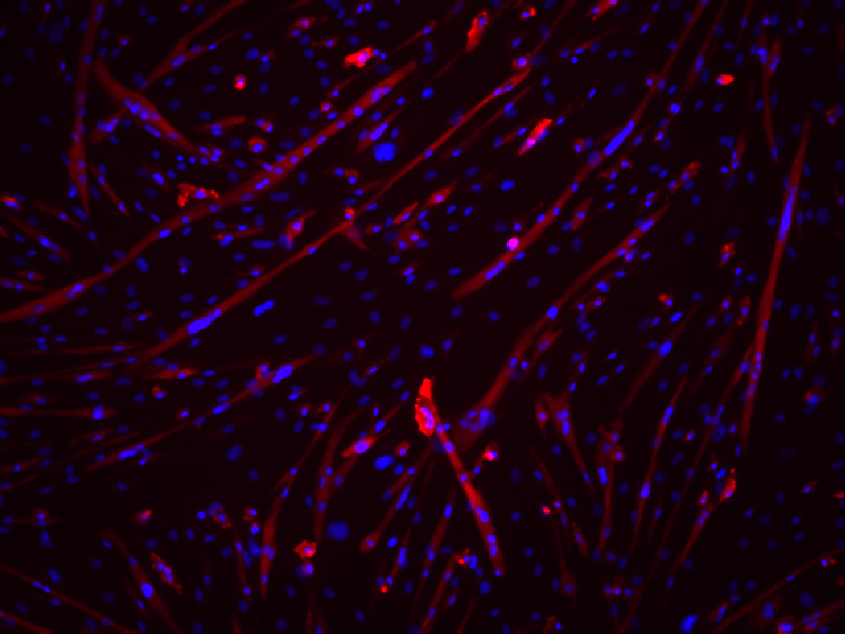
\includegraphics[width=0.45\columnwidth]{figures/myotubes}}
\qquad
\subfloat[][]{\label{subfig:myotubes-analyzed}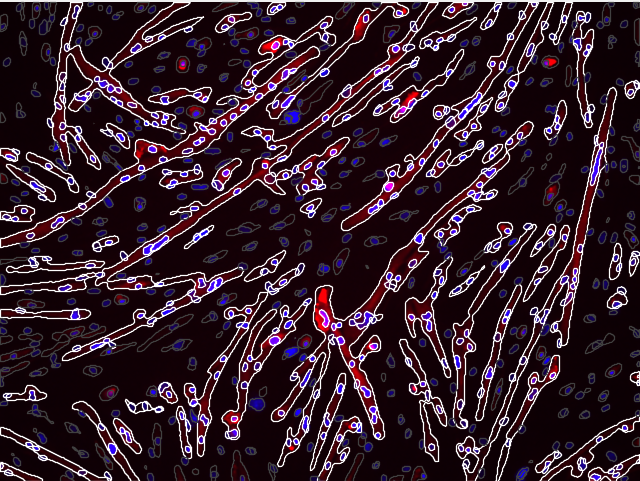
\includegraphics[width=0.45\columnwidth]{figures/myotubes_analyzed}}
\caption{Myoblasts fusing into myotubes \protect\subref{subfig:myotubes-raw}, where the red channel is myosin heavy chain and the blue channel is DAPI. In the analyzed image \protect\subref{subfig:myotubes-analyzed}, myotubes and their nuclei have white outlines and unfused myoblasts and their nuclei have gray outlines. This particular image has a fusion index of 0.54, according to the automated analysis}
\label{fig:myotubes}
\end{center}
\end{figure}

\begin{figure}[!htb]
\begin{center}
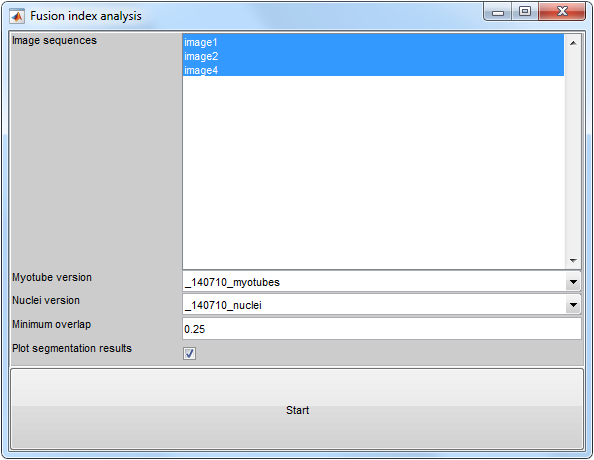
\includegraphics[width = 0.5\columnwidth]{figures/fusionIndexGUI}
\caption{GUI which computes the fusion index of myoblasts that are fusing into myotubes.}
\label{fig:fusion-index-GUI}
\end{center}
\end{figure}

\section{Development}
If you are a biologist and want to analyze the tracks or outlines of cells in a way currently not possible from within the program, or if you are an algorithm developer and want to modify a processing step in the program, you will need to write some code of your own. This section describes how to write custom analysis scrips and explains the basic structure of the program, to make it easier for researchers to make changes to the program.

\subsection{Git}
\label{sec:git}
The BA uses Git for version control. The git software can be installed by following the instructions in Section \ref{sec:install-git}. A Git repository with the version controlled source code is publicly available on \url{https://github.com/klasma/BaxterAlgorithms} and can be downloaded by following the steps in Section \ref{sec:clone}. Once you have downloaded the repository, you can update the source code to the latest version by following the instructions in Section \ref{sec:pull}.

\subsubsection{Installing Git}
\label{sec:install-git}
Git can be downloaded from \url{http://git-scm.com} and information on how to use it can be found at \url{http://gitref.org}. Use the default installation options unless you know what the other options do. On Windows, Git commands can be executed in a program called Git Bash and there is also a graphical user interface called Git GUI. On Mac, Git commands can be executed in the terminal window and Git GUI can be started by typing \command{git gui} in the terminal window.

\subsubsection{Downloading the BA using Git}
\label{sec:clone}
Install Git and open Git Bash on Windows or a terminal window on Mac. Go to the directory where you want to put the software folder, using \command{cd} followed by the directory name. Then type \command{git clone https://\allowbreak github.com/\allowbreak klasma/\allowbreak BaxterAlgorithms.git} to make a copy of the BA repository on your computer. You can paste text into Git Bash using \command{Shift+Insert}. The downloaded project is a normal folder containing the program files, but it also contains a hidden folder named \file{.git}, where all information connected to version handling is stored.

\subsubsection{Updating the BA using Git}
\label{sec:pull}
To update the BA, you do not need to clone the project again. Instead, you can use the Git command \command{git pull origin master}. This command, and all other Git commands except \command{git clone}, must be issued from within the project repository. To go there, you use the command \command{cd} followed by the path of the repository. If you have edited files that would be overwritten by an update, Git will notify you and tell you what your options are.

\subsection{Structure of the repository}
The Git repository contains files and folders. The files which are not inside a folder can be executed on their own, while the files in the folders are executed from other files. Table \ref{tab:files} describes the files in the root directory of the repository, and Table \ref{tab:folders} describes the folders.

%The file \file{BaxterAlgorithms.m} creates the main window from which all other GUIs can be opened. The file \file{BaxterAlgorithmsTerminal.m} runs the cell tracking without opening a GUI. The file \file{CompileMex.m} compiles C++ code used by the program into mex-files that can be executed by MATLAB. The file \file{BaxterAlgorithms.prj} is a deployment project which can be used to create a Baxter Algorithms executable which can be executed without a MATLAB license. The deployment process is described in Section \ref{sec:deploy}. The file \file{startup.m} is executed every time MATLAB is started in the repository. The code in the file adds all of the folders in the repository to the MATLAB path, so that all of the files inside them can be found when MATLAB tries to execute them. The folders are also added to the MATLAB	path by \file{BaxterAlgorithms.m}, \file{BaxterAlgorithmsTerminal.m}, \file{CompileMex.m}, so in general, you do not need to execute \file{startup.m} manually if MATLAB is not started in the repository. That is however necessary before you deploy the software using \file{BaxterAlgorithms.prj}.

\begin{table}[!htbp]
\caption{Files in the root directory of the repository.}
\label{tab:files}
\begin{tabularx}{\textwidth}{lX}
\hline
.gitignore & Specifies a set of files which are excluded from version control.\\[5pt] \hline

AnalysisExample.m & Simple example of a custom analysis script.\\[5pt] \hline

BaxterAlgorithms.m & Creates the main window from which all other GUIs can be opened.\\[5pt] \hline

BaxterAlgorithms.prj & Deployment project which can be used to create a Baxter Algorithms program which can be executed without a MATLAB license. The deployment process is described in Section \ref{sec:deploy}.\\[5pt] \hline

BaxterAlgorithmsTermial.m &  Runs the cell tracking without opening a GUI.\\[5pt] \hline

CompileMex.m &  Compiles C++ code used by the program into mex-files that can be executed by MATLAB.\\[5pt] \hline

LICENSE.md & License file which specifies the terms under which the software may be used.\\[5pt] \hline

README.md & Short information about how the software can be used.\\[5pt] \hline

startup.m &  A script which is executed every time MATLAB is started in the repository. The script adds all of the folders in the repository to the MATLAB path, so that all of the files inside them can be found when MATLAB tries to execute them. The folders are also added to the MATLAB	path by \file{BaxterAlgorithms.m}, \file{BaxterAlgorithmsTerminal.m}, and \file{CompileMex.m}, so in general, you do not need to execute \file{startup.m} manually if MATLAB is not started in the repository. That is however necessary before you deploy the software using \file{BaxterAlgorithms.prj}.\\[5pt] \hline
\end{tabularx}
\end{table}

%The folder \file{Analysis} contains functions for data analysis and plotting. The folders \file{ImageData}, \file{Cell}, and \file{Blob} contain files related to the data classes described in Sections \ref{sec:imagedata}, \ref{sec:cell}, and \ref{sec:blob}. All external code has been placed in the folder \file{External}, together with the respective license files. The folder \file{Files} contains all non-executable files which are used by the program, except this user guide. This user guide and the files which have been used to create it can be found in the folder \file{UserGuide}. The release notes are located in the folder \file{ReleaseNotes}. The folder \file{GUIs} contains most of the code for the graphical user interfaces. The folder PerformanceEvaluation contains the code and the GUIs which are used to compute the segmentation and tracking performance measures SEG and TRA. The folder \file{Preprocessing} contains functions which are used to preprocess the images before the segmentation algorithms are applied. The folder \file{Scores} contains code to compute tracking scores for different cell counts in segmented regions, and events such as mitosis and cell death. The folders \file{Segmentation} and \file{Tracking} contain code to perform image segmentation and track linking respectively. The folder \file{Settings} contains code to keep track of and manipulate parameters which are used by the different algorithms. The folder \file{Utilities} contains low level help functions which are used by many other parts of the program.

\begin{table}[!htbp]
\caption{The contents of folders in the root directory of the repository.}
\label{tab:folders}
\begin{tabularx}{\textwidth}{lX}
\hline
Analysis &  Functions for data analysis and plotting.\\[5pt] \hline

Blob & The class Blob, which represents cell outlines, and functions that operate on the class. See Section \ref{sec:blob} for more information.\\[5pt] \hline

Cell &  The class Cell, which represents cell tracks, and functions that operate on the class. See Section \ref{sec:cell} for more information.\\[5pt] \hline

External & External code and the corresponding license files.\\[5pt] \hline

Files & All non-executable files which are used by the program, except this user guide.\\[5pt] \hline

GUIs & Most of the code for the graphical user interfaces.\\[5pt] \hline

ImageData & The class ImageData, which represents image sequences, and functions that operate on the class. See Section \ref{sec:imagedata} for more information.\\[5pt] \hline

PerformanceEvalution & Code and GUIs which are used to compute the segmentation and tracking performance measures SEG and TRA.\\[5pt] \hline

Preprocessing & Functions which are used to preprocess the images before the segmentation algorithms are applied.\\[5pt] \hline

ReleaseNotes & Release notes for the BA.\\[5pt] \hline

Scores & Code to compute tracking scores for different cell counts in segmented regions, and events such as mitosis and cell death.\\[5pt] \hline

Segmentation & Code to find the outlines of cells.\\[5pt] \hline

Settings & Code to keep track of and manipulate parameters which are used by the different algorithms.\\[5pt] \hline

Tracking & Code to link cell outlines into tracks.\\[5pt] \hline

UserGuide & This user guide and the files which were used to create it.\\[5pt] \hline

Utilities & Low level help functions.\\[5pt] \hline
\end{tabularx}
\end{table}

\subsection{Structure of the data}
The outlines and the tracks of the cells are stored in mat-files in subfolders of the experiment's \file{Analysis} folder, with names that start with \file{CellData}. The cell data associated with an image sequence can be loaded using the function \command{LoadCells}, and saved using the function \command{SaveCells}. The following subsections explain the three classes, \command{ImageData}, \command{Cell}, and \command{Blob}, which are used to store information about the image sequences, the cells, and the outlines of the cells respectively.

\subsubsection{ImageData}
\label{sec:imagedata}
The ImageData class is located in \file{ImageData/\allowbreak ImageData.m} and is used to store information about image sequences.

\subsubsection{Cell}
\label{sec:cell}
The cell class is located in \file{Cell/\allowbreak Cell.m} and is used to store information about the individual cells. When a cell undergoes mitosis, the program ends that Cell object and creates two new Cell objects for the child cells. The Cell objects have the fields \setting{parent} and \setting{children} which store pointers of the Cell objects of the parent and the children of the cell respectively. The $x$-, $y$- and $z$-coordinates  of the cell centroids at different time points are stored in the fields \setting{cx}, \setting{cy}, and \setting{cz} and the outlines at different time points are stored as an array of Blob objects in the field \setting{blob}. The field \setting{firstFrame} specifies the first frame that the cell appears in and the field \setting{lifeTime} specifies the number of frames that the cell appears in.

\subsubsection{Blob}
\label{sec:blob}
A Blob object stores information about a cell outline. For 2D data, the field \setting{image} is a binary sub-image of the smallest possible size, where cell pixels are 1's and background pixels are 0's. The field \setting{boundingBox} is a 4 element array specifying where in the original image the sub-image is located. For 3D data, \setting{image} is a binary 3D array and \setting{boundingBox} is a 6 element array which specifies the location of the 3D array in the original $z$-stack.

\subsection{Documentation}
To get more information about a function or a class, you can type \command{help} or \command{doc} followed by the name of the function or class in MATLAB's command window. The \command{help} command displays information directly in the command window while the \command{doc} command displays a formatted version of the information in a separate window. The m-file of the function or class needs to be on the MATLAB path for the \command{help} and \command{doc} commands to work.

\subsection{Writing custom analysis scripts}
The BA has many built in function for data analysis, but if you want a readout which is not available, you can easily write analysis scrips of your own in MATLAB. The following example script plots the number of cells in an image sequence as a function of time.
% caption=A MATLAB script which plots the number of cells in an image sequence as a function of time.
\begin{lstlisting}[language=Matlab]
% Path of the image sequence folder.
seqPath = 'C:/ExperimentFolder/ImageSequenceFolder';

% Object with data about the image sequence.
imData = ImageData(seqPath);
% Load outlines and tracks of cells saved
% in the folder CellData_label.
cells = LoadCells(seqPath, '_label');
% Remove debris.
cells = AreCells(cells);

% Time points in hours.
t = (0:imData.sequenceLength-1) * imData.dT / 3600;
% The number of cells at each time point.
numberOfCells = zeros(imData.sequenceLength,1);
for i = 1:length(cells)
    ff = cells(i).firstFrame;
    lf = cells(i).lastFrame;
    % Increase the cell count.
    numberOfCells(ff:lf) = numberOfCells(ff:lf) + 1;
end

% Plot the cell counts.
figure
plot(t, numberOfCells, 'LineWidth', 2)
xlabel('time (hours)')
ylabel('number of cells')
ylim([0 16])  % Change the limits on the y-axis.
\end{lstlisting}
Figure \ref{fig:count-plot} shows the plot produced by the above script, for an image sequence with 14 cells at the end.

\begin{figure}[!htb]
\begin{center}
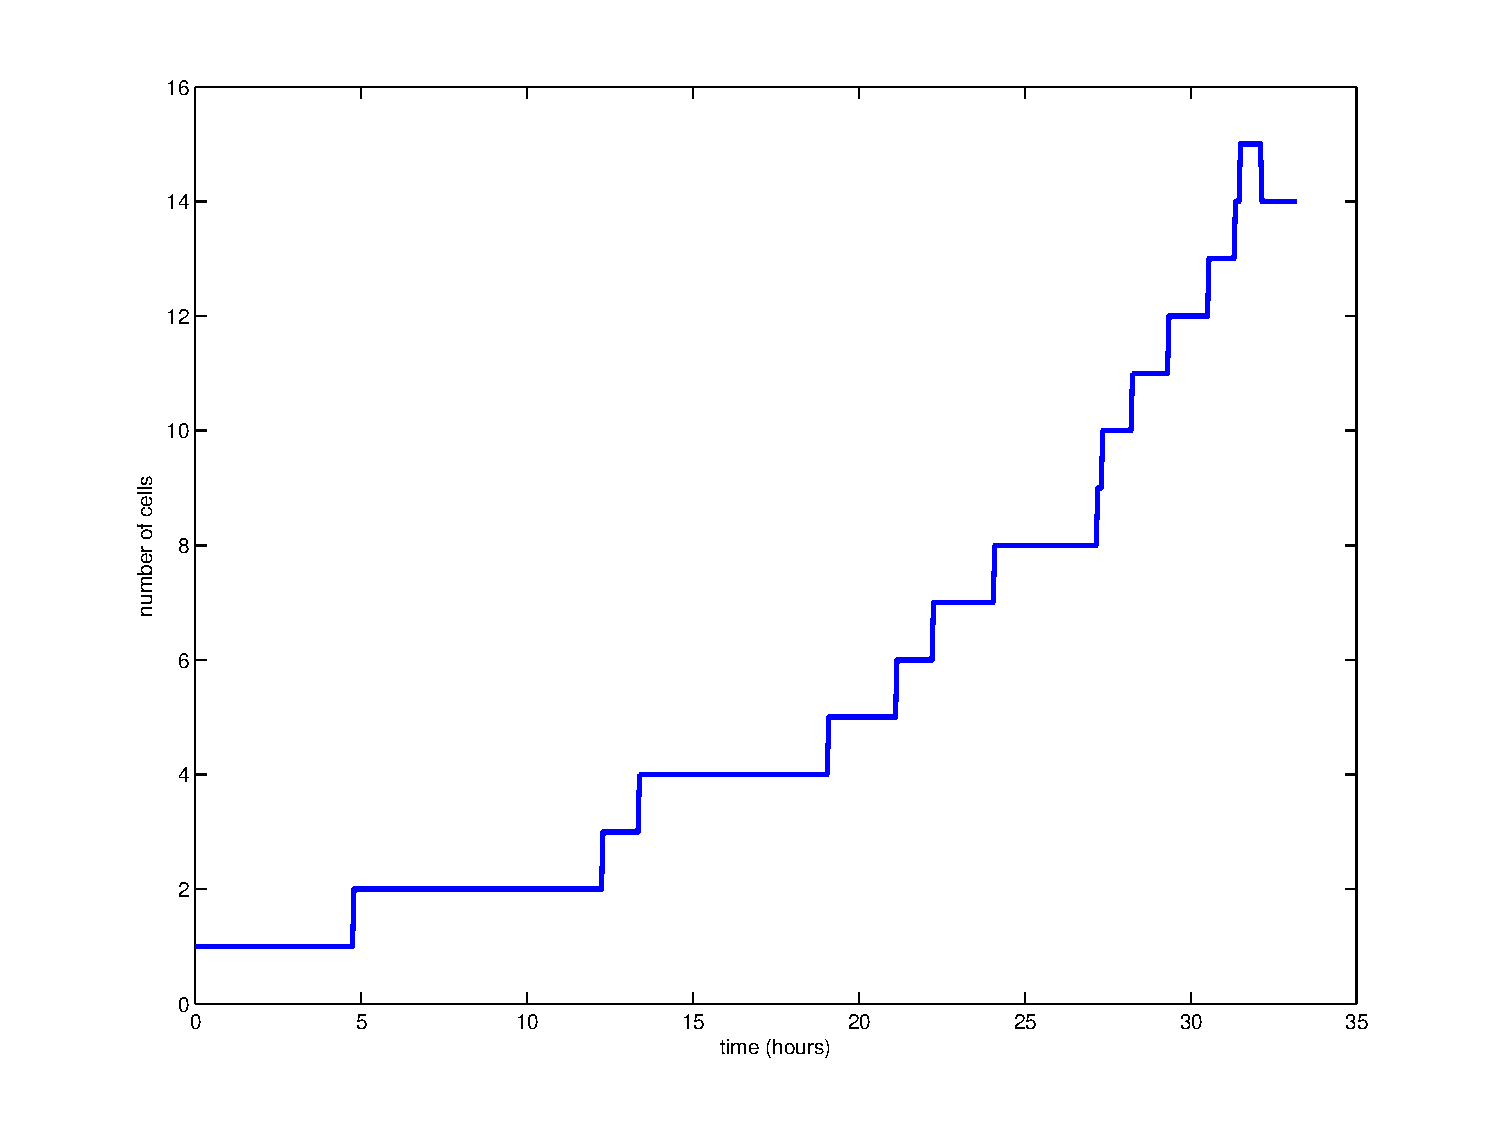
\includegraphics[width = 0.75\columnwidth]{figures/countPlot}
\caption{Plot of the number of cells in an image sequence as a function of time.}
\label{fig:count-plot}
\end{center}
\end{figure}

\subsection{Adding a new segmentation algorithm}
If you cannot find a good segmentation algorithm in the segmentation GUI described in Section \ref{sec:segmentation-gui}, you can add a segmentation algorithm of your own to the program. To do this, you need to write a MATLAB function that takes a grayscale image as input and outputs a binary segmentation mask where foreground pixels are 1's. Then you need to add the function to the files \file{Segmentation/\allowbreak Segment\_generic.m} and \file{Settings/\allowbreak AllSettings.m}.

\subsection{External components}
\label{sec:external}
The BA uses a number of functions that have been developed by others. The functions and their respective licenses are listed in Table \ref{tab:external}. The external code and the licenses can be found in the directory \file{External} in the root directory of the Git repository. The contents of the license files can also be viewed in Section \ref{sec:licenses}. In cases where modifications have been made, the modifications are released under the MIT license as specified in the license file in the root directory of the Git repository.

\begin{table}[!htbp]
\caption{External code components written by others.}
\label{tab:external}
\begin{tabularx}{\textwidth}{llX}
Name & License & Description\\
\hline
bwdistsc & BSD (2 clause) & Computes Euclidean distance transforms of binary 3D images with non-isotropic voxel aspect ratios. Copyright 2007 Yuriy Mishchenko.\\
getGitInfo & BSD (2 clause)  & Returns information about the current branch and commit in a Git repository. The inputs and outputs have been modified.  Copyright 2011 Andrew Leifer.\\
medfilt3 & BSD (2 clause) & Performs median filtering of 3D arrays. Copyright 2011 Simon Robinson and 2014 Jimmy Shen.\\
ParforProgMon & BSD (3 clause) & A progress bar which can be used in a parfor loop. Copyright 2009 The MathWorks, Inc. and 2011 Willem-Jan de Goeij.\\
plotboxpos & MIT & Returns the position of an axes object inside a figure. Copyright 2015 Kelly Kearney.\\
uigetfile\_n\_dir & BSD (2 clause) & The original function is used to select multiple files and directories. A modified version which only selects multiple directories is used in the BA. Copyright 2011 Peugas.\\
\end{tabularx}
\end{table}

\subsection{Compiled C++ code}
\label{sec:compile}
The program contains some compiled C++ functions. The functions have been compiled for 64-bit Windows and 64-bit Mac, but if you are using a different operating system or if you make changes to the C++ code, you will need to compile the functions into mex-files. This is done using the function \command{CompileMex}.

In order to compile mex files with \command{CompileMex}, you need to have a C++ compiler installed and tell MATLAB to use the compiler by running the command \command{mex -setup}. On Mac you can get a C++ compiler by installing Xcode from \url{https://developer.apple.com/xcode/}. In order to use the compiler, you may also need to install command line tools for Xcode, which can be done from within Xcode. On Windows, you can get a C++ compiler by installing Visual Studio Express.

\subsection{Deploying the BA}
\label{sec:deploy}
Users who do not have a MATLAB license can use a deployed version of the BA. Deployed versions can be downloaded and installed for 64-bit Windows and Mac, by following the instructions in Section \ref{sec:run-deployed}. For other operating systems, there are no deployed versions available. To create a deployed version, you need to have a MATLAB Compiler license and have MATLAB installed, together with the toolboxes needed by the BA, on the type of operating system that you want to deploy for. Before you deploy the BA, you need to make sure that all program folders are on the MATLAB path by opening the root directory of the program and running \file{setup.m}. To deploy the program, you open the file \file{BaxterAlgorithms.prj} by double clicking it in MATLAB. Then you press the \control{Package} button. This creates an installer file in a new folder named \file{BaxterAlgorithms/for\_redistribution}. On 64-bit Windows, the file is called \file{BaxterAlgorithmsInstaller\_win64.exe}, and on 64-bit Mac it is called \file{BaxterAlgorithmsInstaller\_maci64.app}. When the installer is executed, it installs the BA and also downloads and installs the MATLAB Compiler Runtime if it is not already installed. The MATLAB Compiler Runtime is a free software which can run deployed MATLAB programs.

\section{How to cite}
If you use the software for a biological study, please site \cite{Magnusson16Thesis}, which describes the software in detail. Use \cite{Magnusson15Viterbi} to cite the track linking algorithm used by the BA, and use \cite{Ulman17Objective} if you want a citation describing the performance of the BA in the Cell Tracking Challenges.

\section{Solving problems}
Bugs related to unexpected inputs or user operations can sometimes cause problems in the program and sometimes the program will not work properly afterwards. To recover from such problems, first try restarting the program and then try restarting MATLAB.

\section{Support}
Please post bug reports, feature requests, and enhancement requests on \url{https://github.com/klasma/BaxterAlgorithms/issues}. When you report a bug, please make sure that you include the MATLAB version, the operating system, the MATLAB error message, and step by step instructions on how to reproduce the bug. Also say whether or not you are running a deployed version of the software.

If you have a question that you cannot find the answer to in this user guide, you can email it to klasmagnus@gmail.com.

\section{Acknowledgements}
The software was developed by Klas Magnusson in a collaboration between the Department of Signal Processing at KTH in Sweden and the Blau Lab at Stanford University in California, USA. Klas was supervised by Joakim Jald\'{e}n at KTH and Helen Blau at Stanford University. In the beginning of the project, Klas was advised by Sebastian Thrun at Stanford University. The idea to automate cell tracking in the Blau Lab came from Karen Havenstrite, and together with Penney Gilbert, she was the first to use an early version of the software in a biological study. The idea to automate the analysis of fluorescently labeled histological sections of muscle came from Andrew Ho in the Blau Lab. The software is named after the Baxter International Foundation, which provided initial funding to start the project. Code contributions have been made by Andrew Chan, who improved graphical user interfaces, and by Colin Holbrook, who made enhancements based on his own user experience. Many others have made important contributions by testing the software and applying it to new types of data.

\section{Licenses}
\label {sec:licenses}
This Section contains the contents of all license files, so that they are not separated from the software when it is released in binary form. The BA is released under the MIT license. The license file is located in the root directory of the Git repository. Section \ref{sec:ba-license} shows the contents of the license file. The contents of the license files of the external components described in Section \ref{sec:external} are shown in Sections \ref{sec:bwdistsc-license} - \ref{sec:uigetfile}. The actual license files can be found in the respective subfolders in the \file{External} directory in the root directory of the Git repository. Note that all modifications to the external components are released under the MIT license.

\subsection{License for BA}
 \label{sec:ba-license}

\begingroup
\footnotesize
\begin{verbatim}
MIT License

Copyright (c) 2018 Klas Magnusson

Permission is hereby granted, free of charge, to any person obtaining a copy
of this software and associated documentation files (the "Software"), to deal
in the Software without restriction, including without limitation the rights
to use, copy, modify, merge, publish, distribute, sublicense, and/or sell
copies of the Software, and to permit persons to whom the Software is
furnished to do so, subject to the following conditions:

The above copyright notice and this permission notice shall be included in all
copies or substantial portions of the Software.

THE SOFTWARE IS PROVIDED "AS IS", WITHOUT WARRANTY OF ANY KIND, EXPRESS OR
IMPLIED, INCLUDING BUT NOT LIMITED TO THE WARRANTIES OF MERCHANTABILITY,
FITNESS FOR A PARTICULAR PURPOSE AND NONINFRINGEMENT. IN NO EVENT SHALL THE
AUTHORS OR COPYRIGHT HOLDERS BE LIABLE FOR ANY CLAIM, DAMAGES OR OTHER
LIABILITY, WHETHER IN AN ACTION OF CONTRACT, TORT OR OTHERWISE, ARISING FROM,
OUT OF OR IN CONNECTION WITH THE SOFTWARE OR THE USE OR OTHER DEALINGS IN THE
SOFTWARE.
\end{verbatim}
\endgroup

\subsection{License for bwdistsc}
\label{sec:bwdistsc-license}

\begingroup
\footnotesize
\begin{verbatim}
Copyright (c) 2007, Yuriy Mishchenko
All rights reserved.

Redistribution and use in source and binary forms, with or without
modification, are permitted provided that the following conditions are
met:

    * Redistributions of source code must retain the above copyright
      notice, this list of conditions and the following disclaimer.
    * Redistributions in binary form must reproduce the above copyright
      notice, this list of conditions and the following disclaimer in
      the documentation and/or other materials provided with the distribution

THIS SOFTWARE IS PROVIDED BY THE COPYRIGHT HOLDERS AND CONTRIBUTORS "AS IS"
AND ANY EXPRESS OR IMPLIED WARRANTIES, INCLUDING, BUT NOT LIMITED TO, THE
IMPLIED WARRANTIES OF MERCHANTABILITY AND FITNESS FOR A PARTICULAR PURPOSE
ARE DISCLAIMED. IN NO EVENT SHALL THE COPYRIGHT OWNER OR CONTRIBUTORS BE
LIABLE FOR ANY DIRECT, INDIRECT, INCIDENTAL, SPECIAL, EXEMPLARY, OR
CONSEQUENTIAL DAMAGES (INCLUDING, BUT NOT LIMITED TO, PROCUREMENT OF
SUBSTITUTE GOODS OR SERVICES; LOSS OF USE, DATA, OR PROFITS; OR BUSINESS
INTERRUPTION) HOWEVER CAUSED AND ON ANY THEORY OF LIABILITY, WHETHER IN
CONTRACT, STRICT LIABILITY, OR TORT (INCLUDING NEGLIGENCE OR OTHERWISE)
ARISING IN ANY WAY OUT OF THE USE OF THIS SOFTWARE, EVEN IF ADVISED OF THE
POSSIBILITY OF SUCH DAMAGE.
\end{verbatim}
\endgroup

\subsection{License for getGitInfo}

\begingroup
\footnotesize
\begin{verbatim}
Copyright (c) 2011, Andrew
All rights reserved.

Redistribution and use in source and binary forms, with or without
modification, are permitted provided that the following conditions are
met:

    * Redistributions of source code must retain the above copyright
      notice, this list of conditions and the following disclaimer.
    * Redistributions in binary form must reproduce the above copyright
      notice, this list of conditions and the following disclaimer in
      the documentation and/or other materials provided with the distribution

THIS SOFTWARE IS PROVIDED BY THE COPYRIGHT HOLDERS AND CONTRIBUTORS "AS IS"
AND ANY EXPRESS OR IMPLIED WARRANTIES, INCLUDING, BUT NOT LIMITED TO, THE
IMPLIED WARRANTIES OF MERCHANTABILITY AND FITNESS FOR A PARTICULAR PURPOSE
ARE DISCLAIMED. IN NO EVENT SHALL THE COPYRIGHT OWNER OR CONTRIBUTORS BE
LIABLE FOR ANY DIRECT, INDIRECT, INCIDENTAL, SPECIAL, EXEMPLARY, OR
CONSEQUENTIAL DAMAGES (INCLUDING, BUT NOT LIMITED TO, PROCUREMENT OF
SUBSTITUTE GOODS OR SERVICES; LOSS OF USE, DATA, OR PROFITS; OR BUSINESS
INTERRUPTION) HOWEVER CAUSED AND ON ANY THEORY OF LIABILITY, WHETHER IN
CONTRACT, STRICT LIABILITY, OR TORT (INCLUDING NEGLIGENCE OR OTHERWISE)
ARISING IN ANY WAY OUT OF THE USE OF THIS SOFTWARE, EVEN IF ADVISED OF THE
POSSIBILITY OF SUCH DAMAGE.
\end{verbatim}
\endgroup

\subsection{License for medfilt3}

\begingroup
\footnotesize
\begin{verbatim}
Copyright (c) 2011, Simon Robinson
Copyright (c) 2014, Jimmy Shen
All rights reserved.

Redistribution and use in source and binary forms, with or without
modification, are permitted provided that the following conditions are
met:

    * Redistributions of source code must retain the above copyright
      notice, this list of conditions and the following disclaimer.
    * Redistributions in binary form must reproduce the above copyright
      notice, this list of conditions and the following disclaimer in
      the documentation and/or other materials provided with the distribution

THIS SOFTWARE IS PROVIDED BY THE COPYRIGHT HOLDERS AND CONTRIBUTORS "AS IS"
AND ANY EXPRESS OR IMPLIED WARRANTIES, INCLUDING, BUT NOT LIMITED TO, THE
IMPLIED WARRANTIES OF MERCHANTABILITY AND FITNESS FOR A PARTICULAR PURPOSE
ARE DISCLAIMED. IN NO EVENT SHALL THE COPYRIGHT OWNER OR CONTRIBUTORS BE
LIABLE FOR ANY DIRECT, INDIRECT, INCIDENTAL, SPECIAL, EXEMPLARY, OR
CONSEQUENTIAL DAMAGES (INCLUDING, BUT NOT LIMITED TO, PROCUREMENT OF
SUBSTITUTE GOODS OR SERVICES; LOSS OF USE, DATA, OR PROFITS; OR BUSINESS
INTERRUPTION) HOWEVER CAUSED AND ON ANY THEORY OF LIABILITY, WHETHER IN
CONTRACT, STRICT LIABILITY, OR TORT (INCLUDING NEGLIGENCE OR OTHERWISE)
ARISING IN ANY WAY OUT OF THE USE OF THIS SOFTWARE, EVEN IF ADVISED OF THE
POSSIBILITY OF SUCH DAMAGE.
\end{verbatim}
\endgroup

\subsection{License for ParforProgMon}

\begingroup
\footnotesize
\begin{verbatim}
Copyright (c) 2011, Willem-Jan de Goeij
Copyright (c) 2009, The MathWorks, Inc.
All rights reserved.

Redistribution and use in source and binary forms, with or without
modification, are permitted provided that the following conditions are
met:

    * Redistributions of source code must retain the above copyright
      notice, this list of conditions and the following disclaimer.
    * Redistributions in binary form must reproduce the above copyright
      notice, this list of conditions and the following disclaimer in
      the documentation and/or other materials provided with the distribution
    * Neither the name of the The MathWorks, Inc. nor the names
      of its contributors may be used to endorse or promote products derived
      from this software without specific prior written permission.

THIS SOFTWARE IS PROVIDED BY THE COPYRIGHT HOLDERS AND CONTRIBUTORS "AS IS"
AND ANY EXPRESS OR IMPLIED WARRANTIES, INCLUDING, BUT NOT LIMITED TO, THE
IMPLIED WARRANTIES OF MERCHANTABILITY AND FITNESS FOR A PARTICULAR PURPOSE
ARE DISCLAIMED. IN NO EVENT SHALL THE COPYRIGHT OWNER OR CONTRIBUTORS BE
LIABLE FOR ANY DIRECT, INDIRECT, INCIDENTAL, SPECIAL, EXEMPLARY, OR
CONSEQUENTIAL DAMAGES (INCLUDING, BUT NOT LIMITED TO, PROCUREMENT OF
SUBSTITUTE GOODS OR SERVICES; LOSS OF USE, DATA, OR PROFITS; OR BUSINESS
INTERRUPTION) HOWEVER CAUSED AND ON ANY THEORY OF LIABILITY, WHETHER IN
CONTRACT, STRICT LIABILITY, OR TORT (INCLUDING NEGLIGENCE OR OTHERWISE)
ARISING IN ANY WAY OUT OF THE USE OF THIS SOFTWARE, EVEN IF ADVISED OF THE
POSSIBILITY OF SUCH DAMAGE.
\end{verbatim}
\endgroup

\subsection{License for plotboxpos}

\begingroup
\footnotesize
\begin{verbatim}
The MIT License (MIT)

Copyright (c) 2015 Kelly Kearney

Permission is hereby granted, free of charge, to any person obtaining a copy of
this software and associated documentation files (the "Software"), to deal in
the Software without restriction, including without limitation the rights to
use, copy, modify, merge, publish, distribute, sublicense, and/or sell copies of
the Software, and to permit persons to whom the Software is furnished to do so,
subject to the following conditions:

The above copyright notice and this permission notice shall be included in all
copies or substantial portions of the Software.

THE SOFTWARE IS PROVIDED "AS IS", WITHOUT WARRANTY OF ANY KIND, EXPRESS OR
IMPLIED, INCLUDING BUT NOT LIMITED TO THE WARRANTIES OF MERCHANTABILITY, FITNESS
FOR A PARTICULAR PURPOSE AND NONINFRINGEMENT. IN NO EVENT SHALL THE AUTHORS OR
COPYRIGHT HOLDERS BE LIABLE FOR ANY CLAIM, DAMAGES OR OTHER LIABILITY, WHETHER
IN AN ACTION OF CONTRACT, TORT OR OTHERWISE, ARISING FROM, OUT OF OR IN
CONNECTION WITH THE SOFTWARE OR THE USE OR OTHER DEALINGS IN THE SOFTWARE.
\end{verbatim}
\endgroup

\subsection{License for uigetfile\_n\_dir}
\label{sec:uigetfile}

\begingroup
\footnotesize
\begin{verbatim}
Copyright (c) 2011, Peugas
All rights reserved.

Redistribution and use in source and binary forms, with or without 
modification, are permitted provided that the following conditions are 
met:

    * Redistributions of source code must retain the above copyright 
      notice, this list of conditions and the following disclaimer.
    * Redistributions in binary form must reproduce the above copyright 
      notice, this list of conditions and the following disclaimer in 
      the documentation and/or other materials provided with the distribution
      
THIS SOFTWARE IS PROVIDED BY THE COPYRIGHT HOLDERS AND CONTRIBUTORS "AS IS" 
AND ANY EXPRESS OR IMPLIED WARRANTIES, INCLUDING, BUT NOT LIMITED TO, THE 
IMPLIED WARRANTIES OF MERCHANTABILITY AND FITNESS FOR A PARTICULAR PURPOSE 
ARE DISCLAIMED. IN NO EVENT SHALL THE COPYRIGHT OWNER OR CONTRIBUTORS BE 
LIABLE FOR ANY DIRECT, INDIRECT, INCIDENTAL, SPECIAL, EXEMPLARY, OR 
CONSEQUENTIAL DAMAGES (INCLUDING, BUT NOT LIMITED TO, PROCUREMENT OF 
SUBSTITUTE GOODS OR SERVICES; LOSS OF USE, DATA, OR PROFITS; OR BUSINESS 
INTERRUPTION) HOWEVER CAUSED AND ON ANY THEORY OF LIABILITY, WHETHER IN 
CONTRACT, STRICT LIABILITY, OR TORT (INCLUDING NEGLIGENCE OR OTHERWISE) 
ARISING IN ANY WAY OUT OF THE USE OF THIS SOFTWARE, EVEN IF ADVISED OF THE 
POSSIBILITY OF SUCH DAMAGE.
\end{verbatim}
\endgroup

\bibliography{refs}

\end{document}
